% \documentclass[11pt,dvipdfm]{article}
\documentclass[11pt]{article}
%\usepackage[utf8]{inputenc}
\usepackage{deauthor,times,graphicx,listings,xcolor,booktabs}
% \usepackage{draftwatermark}

\graphicspath{{submissions/quill-ar-nandi/}}
\definecolor{quillred}{rgb}{0.8, 0.474, 0.655}


\begin{document}
\title{Quill: A Declarative Approach for Accelerating\\ Augmented Reality Application Development}
\author{
Codi Burley, Ritesh Sarkhel, and Arnab Nandi\\
The Ohio State University\\
\{burley.66, sarkhel.5, nandi.9\}@osu.edu
}
\maketitle
\begin{abstract}
Data we encounter in the real-world such as printed menus, business documents, and nutrition labels, are often ad-hoc. Valuable insights can be gathered from this data when combined with additional information.
Recent advances in computer vision and augmented reality have made it possible to understand and enrich such data.
Joining real-world data with remote data stores and surfacing those enhanced results in place, within an augmented reality interface can lead to better and more informed decision-making capabilities. 
However, building end-user applications that perform these joins with minimal human effort is not straightforward. It requires a diverse set of expertise, including machine learning, database systems, computer vision, and data visualization.
To address this complexity, we present \emph{Quill} -- a framework to develop end-to-end applications that model augmented reality applications as a join between real-world data and remote data stores. 
Using an intuitive domain-specific language, Quill accelerates the development of end-user applications that join real-world data with remote data stores.
Through experiments on applications from multiple different domains, we show that Quill not only \textit{expedites} the process of development, but also allows developers to build applications that are \textit{more performant} than those built using standard developer tools, thanks to the ability to optimize declarative specifications.
We also perform a user-focused study to investigate how easy~(or difficult) it is to use Quill for developing augmented reality applications than other existing tools.
Our results show that Quill allows developers to build and deploy applications with a lower technical background than building the same application using existing developer tools.
\end{abstract}

\section{Introduction}
\label{sec:intro}
We gather information in our everyday life not only through digital interfaces such as mobile devices, computers, and wearables, but also through multiple physical media that surround us in the real world, such as movie posters, billboards, chalkboard menus, and grocery lists. Real-world data is diverse and rich in its complexity. It is also \textit{one-size-fits-all} -- unlike digital data which is often personalized or transformed based on the downstream task, we all see the same real-world data irrespective of our information needs. This makes it challenging to devise a generalizable solution to gather insights from real-world data.
For example, if \textit{Alice} wants to find out ``recent reviews of the most popular dish in a newly opened restaurant'', she will need to formulate her information need as a tangible query first, look up the results of that query in a browser-based search engine, and then filter down the returned results to find an appropriate answer. If \textit{Bob} wants to find out the reviews of another dish from the same restaurant, he would have to go through the same steps again. Real-world data is also \emph{incomplete}: it may provide little to no context with respect to the information a consumer may need. For example, restaurant menus often lack supplementary information such as a list of ingredients and allergens present in a dish. As a result, if \textit{Alice} wants to discern if a dish in her favorite restaurant has nuts in it, she has to manually perform what is essentially a join between real-world data, i.e., the name or image of the dish, and a remote data store, i.e., a nutritional database that contains the list of ingredients.
\looseness=-1

\begin{figure}
  \centering
  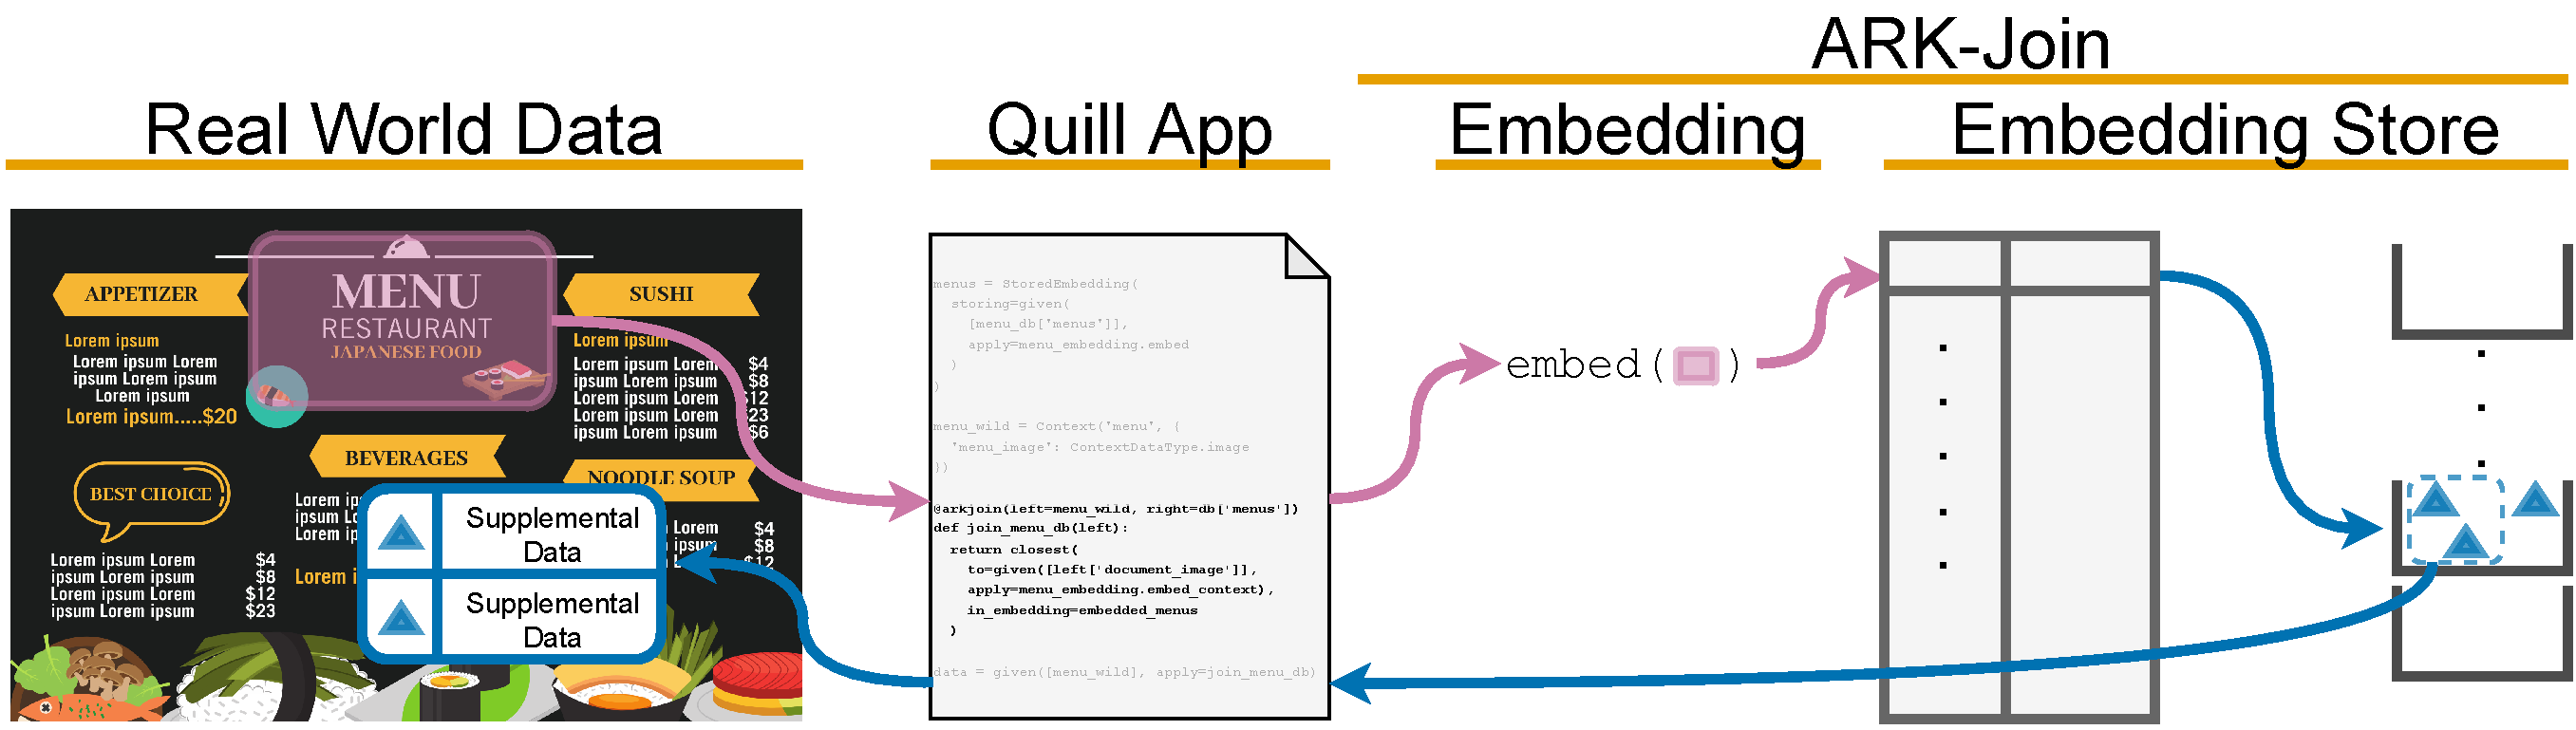
\includegraphics[width=0.94\linewidth]{figs/workflow_large.pdf}
  \caption{This figure demonstrates the flow of an application developed using the \textit{Quill} framework, performing an Augmented Reality-adapted Keyless Join~(ARK-Join). An AR-enabled client sends requests in the form of data elements from a \textit{real-world context} to the Quill app, which is defined using a script written in a domain-specific language, called \textit{QWL}. The ARK-Join operation then finds sufficiently similar data elements from a specified \textit{remote source} by searching over an indexed \textit{embedding store}. Results of this join operation are sent to the client which uses this data to augment the user's view with supplementary information.\looseness=-1}
  \label{fig:overview}

\end{figure}

Augmented reality~(AR), a technology to overlay the physical world with digital information, provides a useful medium for enriching real-world data with supplementary information. The rapid advancement of cameras and computational power in consumer-grade mobile devices~\cite{azuma2001recent} have made AR widely available in recent years. In prior work~\cite{burley2019arquery} titled ``ARQuery'', we have shown that AR can be an effective way to explore real-world data interactively. For example, interactive querying of each dish in the menu through an AR-enabled interface for relevant supplementary information~(e.g., ingredients used, customer reviews) using simple gesture-based interactions~\cite{nandi2013gestural} can be vastly more efficient than manually looking up a browser-based search engine. However, as depicted in the example below, building a robust capability towards joining real-world data through an interactive, AR-enabled view without handcrafted features and minimal human supervision requires extensive machine learning capabilities~\cite{fernandez2018seeping}.
% Furthermore, mobile-based AR devices are battery-bound~\cite{tang2020cooperative} and have serious computational limitations, which make the required computations difficult to be accomplished on-device. Edge computing, a network-enabled computing approach that aims to bring compute resources closer to mobile devices has proven to be useful in addressing these challenges using computation offloading and intelligent caching mechanisms~\cite{drolia2017cachier, li2017mobiqor, ren2018mobile}.
To address these needs, we provide a domain-specific language~(DSL) for defining applications that join real-world data with semantically similar data elements in remote data stores in an easy-to-use framework, called \textit{Quill}.

With Quill, we provide a framework for developing augmented reality applications that enrich the real-world data elements with supplementary information from remote data stores. This framework is centered around an easy-to-use DSL, called \textit{\textbf{Q}uill \textbf{W}orkflow \textbf{L}anguage} or \textit{QWL}. Using QWL, developers can define various task-specific parameters such as the remote data stores to be joined against, data embedding techniques to be used, and more. We describe all such parameters currently supported by Quill in Section III. Quill's framework then produces a ready-to-deploy application that serves input requests in the form of ad-hoc real-world data. It performs this join operation with minimal human supervision and handcrafted features in its end-to-end workflow. This is achieved by comparing remote data elements to incoming real-world data elements in a shared vector space. The DSL also enables us to define various application-specific parameters, e.g., whether to cache previously computed results locally or to recompute them when comparing against a remote data element. We discuss the challenges addressed by our framework in greater detail after describing a scenario that showcases some of these challenges and demonstrates how {Quill} accelerates the development workflow.\looseness=-1\vspace{0.05cm}

\textbf{Example 1.1: } \textit{Alice} is visiting a French cafe. The cafe has a printed menu. \textit{Alice} wants to order an appetizer but wants to know its calorific and allergen information first.
She has to pore through the appetizer section of the menu and manually look up the necessary information for each item one at a time. With an application developed using {Quill}, \textit{Alice} simply views the menu through her phone's live camera view and selects the dish she wishes to know more about in the menu using simple gesture-based interactions. This initiates a join of the real-world data retrieved from the menu, i.e., the dish \textit{Alice} is interested in against a nutritional database. 
Results of this operation are retrieved from the server running the Quill app and rendered as interactive components in \textit{Alice's} live camera view.
Quill enables a developer to create such applications by using a script written in QWL, Quill's DSL. We refer to these applications as Quill apps in the rest of this document. Figure 1 demonstrates the workflow of a typical Quill app. Next, we describe the challenges of developing a framework that enriches real-world data with remote data stores in an augmented reality setting.\looseness=-1\vspace{0.15cm} 

\label{sec:intro:challeneges}

\newcommand{\challengemultimodal}{1}
\textbf{Challenge 1: } Real-world data is multimodal. Consider the scenario in Example 1.1. Previous works~\cite{sarkhel2019deterministic, sarkhel2019visual,sarkhel2021improving} suggest that extracting information such as the name of a dish and its price from a live camera view requires considering both the textual and visual properties of the menu. Therefore, a development framework that enables the enrichment of real-world data captured through camera-enabled AR interfaces will need to account for multiple data modalities.\vspace{0.07cm} 

\newcommand{\challengehetero}{2}
\textbf{Challenge 2: }
Modern data stores are often heterogeneous. Instances that contain structured, unstructured, and semi-structured data elements altogether have become a common occurrence.
Recent works~\cite{suri2021ember,fernandez2019termite,li2021auto} have shown that similarity-based joins such as keyless joins are useful alternatives to traditional join operators for modern data stores due to their heterogeneous nature.
However, previous keyless joins have been restricted to singular domains that do not generalize to all kinds of real-world data.
Quill enables joining real-world data with remote data stores by implementing a \textit{AR-adapted keyless join}~(ARK-join) operation.\looseness=-1 \vspace{0.07cm}

\newcommand{\challengecustom}{3}
\textbf{Challenge 3: } A development framework that enriches real-world data with a remote data store needs to be both \textit{flexible} and \textit{modular}. It should be flexible enough to allow its end-users to define the underlying join operation in a fine-grained way.
For example, for the managers of the restaurants \textit{Alice} visits, enhancing a restaurant menu with supplementary information from the inventory database is more useful to plan ahead and keep the pantry stocked.
Integration of machine learning components into interactive data systems is an active area of research. Therefore, a development framework should also be modular such that new advances in related areas, e.g., keyless joins, data transformation/embedding functions, and indexing techniques, can be seamlessly integrated.\vspace{0.07cm} 

\newcommand{\challengeperform}{4}
\textbf{Challenge 4: }
The framework should be both \textit{easy-to-use} and \textit{performant}. In other words, compared to applications built without Quill, Quill apps should require less development effort without sacrificing accuracy or latency.\looseness=-1 

\subsection{Technical Contributions}
Keeping the above mandates in mind, we describe Quill's main contributions below.\looseness=-1

\begin{itemize}
    
	\item an augmented reality adapted keyless join~(ARK-join) operation to enrich ad-hoc real-world data with heterogeneous data elements from remote data stores,
	
	\item an easy-to-use domain-specific language called QWL that allows users to express task specifications in a fine-grained way~(including details of the architecture where the application will be deployed),
	
	\item a performant framework for developing performant applications that enhance real-world data in a fast and accurate way.
	
\end{itemize}

Quill makes it easier to gather insights from real-world data by accelerating the development workflow of applications that enrich real-world data elements with semantically similar data from remote data stores. By using a keyless join, Quill makes it possible to enrich real-world data in a context-aware way with minimal human intervention and handcrafted feature engineering. Through exhaustive experiments on four real-world applications~(see Section~\ref{sec:evaluation}), we show that developing applications is faster using Quill than other developer tools. Moreover, in Section~\ref{sec:evaluation:usability} we outline how Quill maintains perfomance while remaining usable. We ensure that Quill apps can operate on large remote data stores by indexing data elements in the remote data store to enable faster approximations with tunable accuracy.
% We ensure that Quill apps can cache locally and run on edge servers to bring processing and caching closer to the user for significant performance advantages.
Our experiments show that Quill apps are more accurate and faster in executing the underlying task than similar applications developed using other developer tools.
% Abstracting the underlying data processing operations through an expressive and easy-to-use DSL, Quill makes it easier for developers with limited background knowledge to harness the power of machine learning, computer vision, and edge computing together in a single performant framework.
Our study with a developer audience demonstrates that (a) Quill's DSL is easy to learn, and (b) using Quill led to more succinct codebases while maintaining expressibility and end-to-end performance. Integration of machine learning components in interactive data systems is an active area of research. Fine-grained task specification capabilities afforded by Quill's expressive DSL make it easier for future advances in related areas, e.g., keyless join and embedding techniques, to be seamlessly integrated into Quill's development workflow. We demonstrate this by developing a Quill app that executes a search task over a benchmark text dataset using learned embedding functions from Ember, a recent work by Suri, Ilyas, R{\'e} and Rekastinas~\cite{suri2021ember}~(see Section~\ref{sec:evaluation:modularity}).



\section{Problem Formulation \& Definitions}
\label{sec:problem}

The Quill framework produces a ready-to-deploy application that responds to data enrichment requests by executing an augmented reality-adapted keyless join~(ARK-join) specified using a DSL. We provide a formal definition of the ARK-Join operation in Section~\ref{sec:background:ark}. Quill's DSL, called QWL, is capable of defining applications that perform both simple joins, i.e., joining a real-world data element with a remote cloud store, and complex multi-joins~(see Fig.~\ref{fig:edge-cache}), i.e., joins between real-world data-elements, a local cache,  as well as a remote data store. Before formalizing the problem Quill solves, we define some of its key concepts and related technology first.\looseness=-1

\subsection{Background and Definitions}
\label{sec:background}

\paragraph{Real-world data:}
\label{sec:background:real-world}
All data elements captured in the live camera view of an AR-enabled interface are considered \textit{real-world data}. Real-world data is inherently multimodal.\vspace{0.05cm}

\paragraph{Remotely stored data:}
\label{sec:background:remote}
\textit{Remotely stored data} represent those data elements that are stored in cloud-based data stores separately from the real-world data captured in the live camera view of an AR-enabled interface. For example, in the edge-based architecture shown in Fig.~\ref{fig:edge-cache}, the data stored in the cache on edge as well as the data stored in the cloud are considered remotely stored data. Quill enriches real-world data with remotely stored data using an \textit{ARK-Join operation}.\vspace{0.05cm}

\paragraph{Keyless Join:}
\label{sec:background:keyless}
Quill builds on existing work on keyless join and fuzzy join. A fuzzy join is a commonly used join operator \cite{afrati2012fuzzy, li2011pass, metwally2012v, chen2019customizable, li2021auto} in structured data settings used to identify matching records. It matches two records $r$ and $s$ from two different databases $R$ and $S$ if $sim(s, r) > \theta$, where $sim$ represents a similarity function \cite{manning2008and} and $\theta$ represents a similarity threshold. Among many options, Jaccard similarity, Hamming distance, and Cosine similarity are some of the most common similarity functions used by contemporary researchers. While some recent works~\cite{chen2019customizable} have tried to propose scalable fuzzy join operators, they have largely been domain-specific. Consequently, they do not generalize well for data stores where data elements are heterogeneous. At the same time, a number of recent works have proposed a keyless join operator~\cite{fernandez2019termite, suri2021ember, li2021auto}. It is an extension of the fuzzy join operator that matches two data-elements $r, s$ if $sim(f_{(s)}(s),f_{(r)}(r)) > \theta$, where $f_{(s)}$ and $f_{(r)}$ are transformations of the data-elements $r, s$ to a shared vector-space. The transformation function $f$ is typically learned from previous examples. AutoFuzzyJoin \cite{li2021auto} searches a configuration space of all possible similarity functions ($sim$), input transformations ($f$), and thresholds ($\theta$) to find the optimal configuration. Ember \cite{suri2021ember} and Termite \cite{fernandez2019termite} use machine learning techniques to learn the transformation function $f$, they use cosine similarity as the similarity function. Keyless join operators are more flexible than traditional fuzzy join operators in capturing semantic information of a data element in a heterogeneous data store.\vspace{0.05cm}

\paragraph{ARK-Join:}
\label{sec:background:ark}
To enrich real-world data with remote data stores, Quill employs a keyless join operator, called the augmented reality adapted keyless join or ARK-Join. Summarily, it is a cross-modal keyless join operation extended for augmented reality enabled interfaces. In terms of its basic functionality, ARK-Join is similar to keyless join~\cite{fernandez2019termite, suri2021ember} except it parameterizes the embedding transformation function $f$ as an additional input to the join operator. This allows a developer using the Quill framework the flexibility to define unique transformation functions for data elements from different modalities. %of data they are dealing with, which could be images in the real-world and text in a remote store for example.
In other words, ARK-Join extends the notion of keyless joins beyond data modalities and makes the join operation more generalizable. ARK-Join operator also differs from other existing works on keyless joins such as Ember~\cite{suri2021ember} and Termite~\cite{fernandez2019termite} in its implementation. It takes advantage of AR-specific constraints, such as the small number of objects that users can track simultaneously at the same time, to optimize the ARK-Join operator for data from camera-enabled AR interfaces. We formalize the ARK-Join operator and describe it in greater detail in Section~\ref{sec:grammar}-B.

\begin{figure}
  \centering
  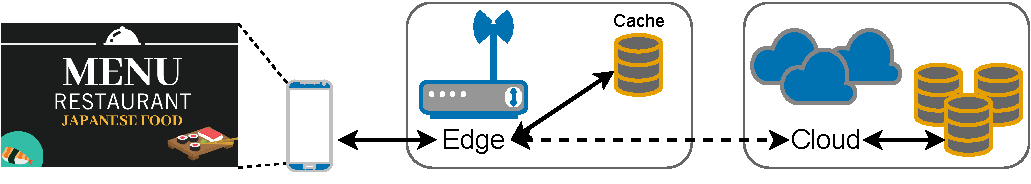
\includegraphics[width=\linewidth]{figs/edge-cache.pdf}
  \caption{A simplified edge-based architecture with an edge cache and a backing cloud store. Quill can produce applications that fit into various architectures such as this one with a single script written in our DSL.}
  \label{fig:edge-cache}
\end{figure}

% \subsubsection{Edge Computing}
% \label{sec:background:edge}
% Edge computing refers to a computational paradigm that brings computing closer to mobile users who will be utilizing the results of the computation, thereby reducing the latency incurred by communication.
% One common use case for edge computing is in retrieval-based applications \cite{drolia2017cachier, li2017mobiqor, ren2018mobile}.
% Figure \ref{fig:edge-cache} provides a high-level overview of an edge architecture used in retrieval based applications. In this example, a mobile device sends a request for information retrieval which is received by the edge server. The edge server contains a cache of results that were previously retrieved from the cloud. If the desired results are contained in the cache (i.e. on a cache hit), the cached results are returned, otherwise (i.e. on a cache miss) the edge server makes a request to the backing cloud store. %Recent works~\cite{drolia2017cachier} have shown that the similarity between incoming requests can be used to determine cache hits in retrieval based applications.
% %We recognize that this similarity based comparison has parallels with the ARK-Join that Quill utilizes.
% In order to minimize end-to-end latency involved in communicating with remote data stores, Quill produces applications that can easily cache locally and thereby take advantage of running on the edge. Upon receiving a request for executing an ARK-Join operation, an application developed using Quill can attempt to fetch pre-computed results from a local cache first. In case of a cache-miss, the join operation is executed on the remote data store and the results are returned back to the user. By placing this cache closer to end-users,  the Quill app takes advantage of edge computing.\vspace{0.05cm}
% %An application with this architecture can be easily defined in a single script written in Quill's DSL.

\paragraph{Quill Apps:}
\label{sec:background:app}
Quill exposes a development framework for applications that enriches real-world data with remote data stores through QWL, an intuitive DSL based on an easy-to-learn grammar (see Section~\ref{sec:grammar}).
We refer to an application produced by Quill's development framework as a \textit{Quill app}. A Quill app is a server application that receives requests to enrich real-world data with semantically similar data elements from remote data stores and responds to these requests by executing an ARK-Join operation (described above) on the remote data store. To develop a Quill app, a developer defines the task specifications and application functionalities using a QWL script. This includes: (a) real-world data provided by the user along with its modality, (b) remote data stores along with methods (e.g. API) for accessing that data, and (c) parameters of the ARK-Join operation which includes the input transformation functions, similarity functions, and similarity threshold. Using the information provided in the QWL script, the Quill framework produces a Quill app.
Based on the composition of ARK-Joins that operate on different data sources, such as local caches and remote cloud stores, Quill can seamlessly produce applications with varying architectures such as the one shown in Fig.~\ref{fig:edge-cache}.\looseness=-1

\subsection{Problem Formulation}
Using the concepts introduced above, we now define the problem that Quill solves. Quill provides a development framework for ready-to-deploy applications that execute ARK-Join operations between real-world and remote data elements in an efficient and effective way. Fig.~\ref{fig:qql-breakdown} shows the DSL script used to define an application that performs an ARK-join to complete the task described in example 1.1. Quill's development framework is centered around an easy-to-learn DSL, called QWL. It is based on a grammar that defines the relation between different components of the application that executes the underlying ARK-join operation. We describe this grammar in Section~\ref{sec:grammar}.



\section{A Grammar for Joining with the Real-World}\label{sec:design:spec}
\label{sec:grammar}

To ensure that our development framework can express a range of different applications, we base our DSL on a grammar that captures the inner workings of all the components that are inherent in an application. We recognize that while general-purpose systems can be designed to perform well for a variety of different applications, tailoring to specific use cases is challenging \cite{jens}. By developing a DSL that is built on an easy-to-learn grammar, we enable the development of such instance-optimized applications for a range of real-world applications. We describe the grammar elements used by Quill's DSL next. They are of three major types: \textit{Data Sources}, \textit{Transformation Functions}, and \textit{ARK-Join Operator}. We finish the section by describing how QWL relates different elements of the grammar using a directed acyclic graph~(DAG).\looseness=-1

\subsection{Data Sources}
In Quill, data sources are collections of data elements of varying modalities that originate from one of the data sources defined by our grammar. Data sources can be both real-world data and remotely stored data as defined in Section~\ref{sec:background}.
We define three different data sources: \emph{Remote Sources}, \emph{Embedding Stores}, and \emph{Real-World Context}.\vspace{0.05cm}

\paragraph{Remote Sources:}
\label{sec:grammar:external}
Remote Sources correspond with remotely stored data~(defined in Section~\ref{sec:background}). Quill apps execute a join operation on data elements from remote sources against real-world data.
Formally, a remote source is comprised of a pair of functions. One function retrieves a collection of data elements~(with identifiers) from the remote store, allowing the data to be embedded and identified.
The other function retrieves a subset of the collection retrieved by the first function that corresponds to a given set of identifiers.\vspace{0.05cm}

\paragraph{Real-World Context:}
Real-world context refers to the real-world data~(defined in Section~\ref{sec:background}) for which we want to gather insights using a Quill app. Real-world context could be an image of a receipt, a transcript, or a restaurant menu. The modality~(e.g., image, text, speech) of the real-world context of an ARK-Join operation is specified in the QWL script. Each definition receives the incoming data elements and triggers corresponding data processing operations to execute the underlying ARK-Join operation as specified in the QWL script.\looseness=-1\vspace{0.05cm}

\paragraph{Embedding Store:}
\label{sec:grammar:embedding_store}
Data elements from both real-world and remote sources are transformed into fixed-length vectors using a transformation function, called embedding functions~(defined below) for an {ARK-Join} operation. Embedded data elements from a remote source are persisted in a data store, called the \textit{embedding store}.
A Quill embedding store comprises a remote data store that contains embedded data elements as fixed-length vectors and an index over those fixed-length vectors. We construct an index over data elements from remote sources for efficient implementation of K-nearest-neighbor-search for executing an ARK-Join operation on large-scale remote sources. We provide a detailed description of the ARK-Join operator in the following section. To construct an embedding store, a developer specifies the embedding function to be used and the indexing scheme as parameters in the QWL script.
A Quill embedding store can be located in the local cache, a large-scale remote data store, or any suitable store reachable from the Quill app.\vspace{0.05cm}

\subsection{Transformation Functions}
Quill supports two major transformation functions: \textit{embedding functions} and \textit{inline transforms}. Data elements from both \emph{real-world context} and \textit{remote sources} are transformed to a shared vector-space to execute the underlying ARK-Join operation. Quill utilizes an \emph{embedding function} for this purpose. Data-elements $r$ and $s$ are joined together if $f_{(r)}$ and $f_{(s)}$ are semantically similar, where $f$ denotes the \textit{embedding function} that encodes data-elements into a fixed-length vector. Generalized \emph{inline transforms}, on the other hand, are used to format the results returned by an ARK-Join operation to be presented back in the live camera view of an AR-enabled interface that the real-world data came from. We describe these transformation functions next.\vspace{0.05cm}

\paragraph{Embedding Functions:}
Quill utilizes embedding functions to transform data elements from the \textit{real-world context} and \textit{remote source} to a fixed-length vector in a shared vector space for the purpose of identifying if a real-world data element is semantically similar to a data element from a remote source. If they are similar, a join operation is executed between the two data elements, and the results are returned back. 
Quill takes embedding functions for each modality of real-world context and remote source used in an app.
\looseness=-1\vspace{0.05cm}

\paragraph{Inline Transforms:}
\label{sec:grammar:inline}
Inline transform functions are responsible for taking the intermediate results returned by an ARK-Join operator and transforming them into a representation that is surfaced back to the client interface.
For example, a built-in inline transform function can take the results of an ARK-Join operation as a dataframe and convert it into a JSON format that is more suitable for representing the results as a table in the live camera-view of an AR-enabled client interface.

\subsection{The ARK-Join Operator}
\label{sec:grammar:ark}
The ARK-Join operator performs a left-outer join between data elements from a \emph{real-world context} and a \textit{remote source}. Data elements from the remote source have already been transformed and stored as fixed-length vectors in an \emph{embedding store}.
As a result of this operation, data elements from the \textit{real-world context}~(i.e., the left operand) are joined with semantically similar data elements~(i.e., the right operand) in the embedding store.
Formally, we define the join predicates of an ARK-Join operation as the $K - n$ \emph{approximate nearest neighbors} of the left operand among the set of right operands, where $0 \ge n \ge K$ is the number of approximate nearest neighbors that are not within similarity threshold $\theta$.
The result-set of this join operation is as follows.
\begin{equation}
\{K\mbox{-}ANN_\theta(x, embed_r(R)) \ : x \in embed_l(L)\}
\end{equation}

\begin{figure}[t]
  \centering
  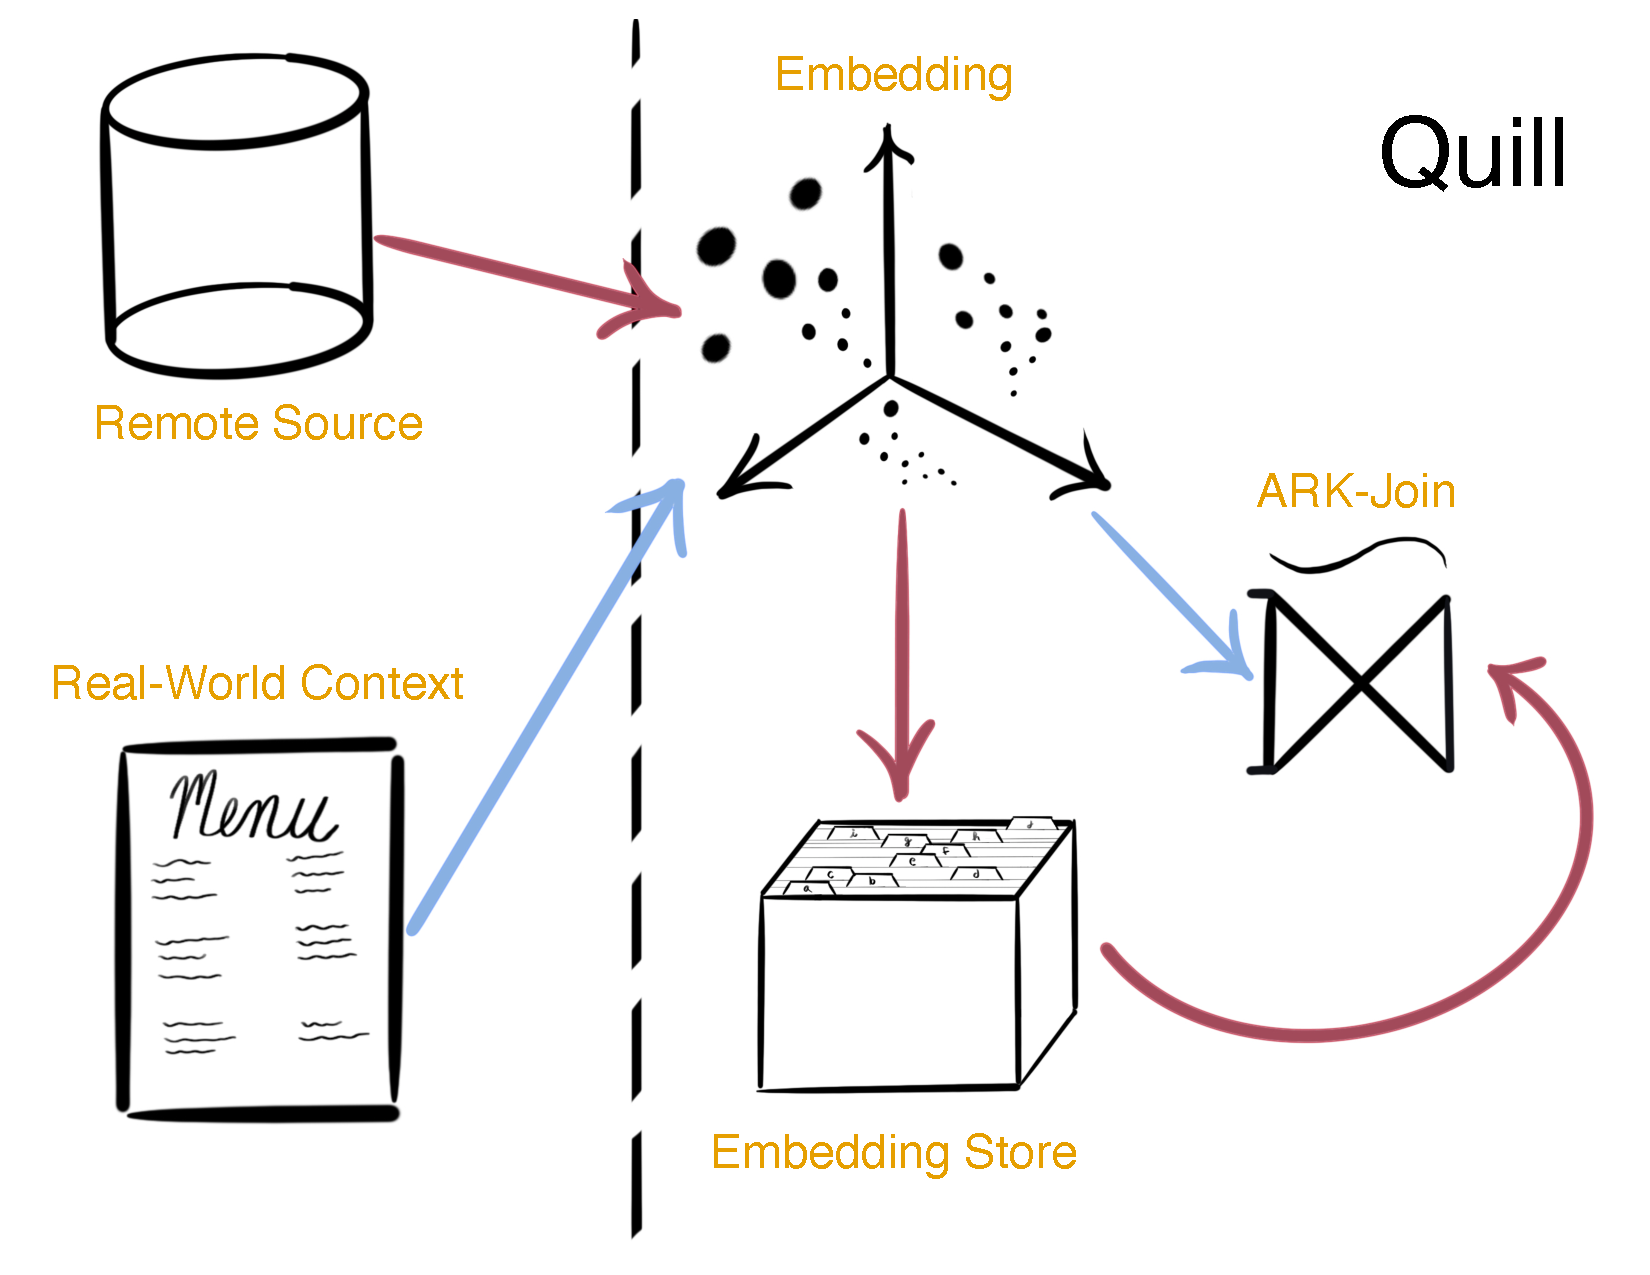
\includegraphics[width=0.6\linewidth]{figs/grammar-w-text.pdf}
  \caption{A high-level view of the grammar used by Quill's development framework. The red color arrows indicate the path data takes from \emph{remote sources} to an \emph{ARK-Join}, while the blue color indicates the path for data from \emph{real-world context}.}
  \label{fig:grammar}
\end{figure}

Where $L$ and $R$ are the left and right operands, the embedding functions $embed_l$, $embed_r$, and $\theta$ and $K$ are specified in a QWL script by the Quill app developer. This join operation retrieves $K - n$ data elements from the remote source $R$ that are most similar to the real-world data element $l$. The use of approximate nearest neighbors in conjunction with the similarity threshold $\theta$ ensures that each left operand is matched with similar tuples, or the null set when no similar tuples (according to $\theta$) are found. Therefore, it can be thought of as a left outer join on real-world data.
Results of this join operation are formatted using \emph{inline transform} functions before being returned back to the user. Contemporary researchers have shown that users have trouble tracking more than four or five objects at a time \cite{cavanagh2005tracking} in a camera-enabled interface.
As we expect the number of incoming requests in the form of data elements from a \textit{real-world context} to be low during each session, it is computationally reasonable to embed real-world data elements on the fly prior to the execution of the join operation. The number of data elements from \emph{remote sources}, on the other hand, can be huge, which motivates the need of constructing an index over the precomputed embedding vectors for each data element in the \emph{embedding store}.

\subsection{QWL: Specifying an ARK-Join using a DSL}
\label{sec:grammar:design}

Internally, scripts written in QWL define a directed acyclic graph~(DAG) between nodes that represent various event-driven elements of the grammar described above. The edges represent dependency relations amongst the nodes. Each node in the graph defines its own execution plan which either: (a) produces data if it is a \textit{data source}-type element, or (b) transforms data if it is a \textit{transformation function}-type element. The execution plan for a node is evaluated when either input from a client triggers the evaluation, or a node on which its query plan depends on has been evaluated. We describe how a QWL script defines relations between different grammar elements next.\vspace{0.05cm} 

\begin{figure}
    \centering
    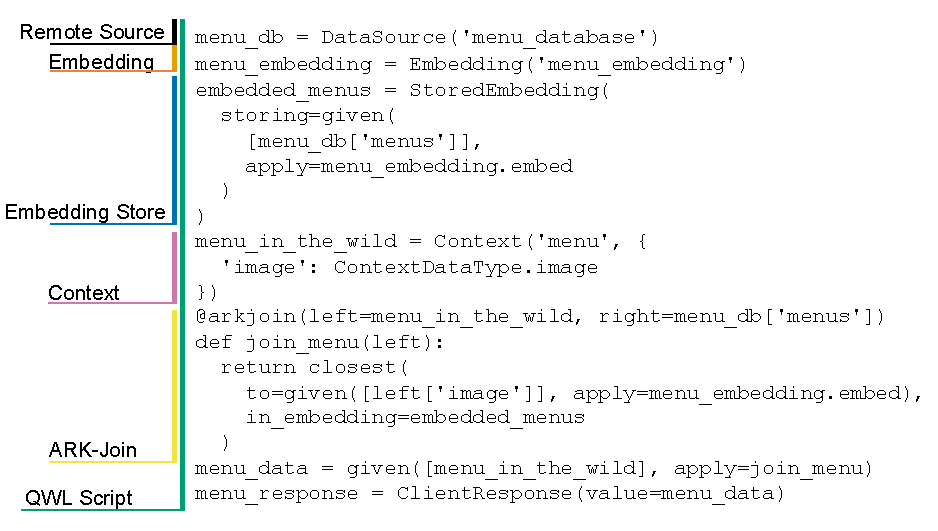
\includegraphics[width=0.7\linewidth,]{figs/annotated_qql_large.pdf}
    \caption{A snippet of the Python QWL interface for specifying Quill applications. This example uses an ARK-Join to retrieve data on a menu from a remote data source that corresponds to a real-world menu instance. 
    }
    \label{fig:qql-breakdown}
\end{figure}

\begin{figure}[t]
    \centering
    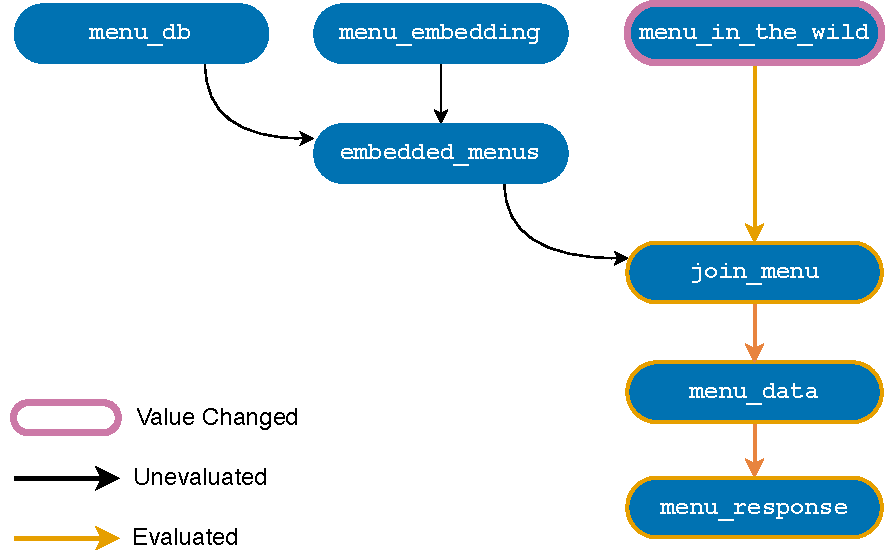
\includegraphics[width=0.6\linewidth]{figs/qql-dependency.pdf}
    \caption{This figure presents the dependency sub-graph relevant to the QWL code presented in Figure \ref{fig:qql-breakdown}.
    The graph shows the evaluation that occurs when data from the \texttt{Menu} is posted  from the client. Quill evaluates declarations that depend on data from the \texttt{Menu} once the input data is posted.}
    \label{fig:dependency}
\end{figure}

QWL relates different grammar elements by using a function application construct, called \emph{waited application}. A waited application lazily evaluates a node's execution plan based on when the nodes it depends on are available~(i.e., not waiting) and all given conditions are met. For example, the evaluation of a node representing a \textit{real-world context} can start after an AR-enabled client interface has detected a gesture-based query that sends data that should be joined to the Quill app in a request. By default, nodes in the DAG that are of \emph{real-world context}-type are waiting, and thus all their dependents are waiting as well. A waited application relates data sources and transformation functions by taking both as inputs and evaluating the results after applying the transformation functions to the data sources. In QWL we use the \texttt{given} function to achieve the functionality of a waited application. Fig.~\ref{fig:qql-breakdown} shows an example QWL script. Fig.~\ref{fig:dependency} shows it corresponding DAG representation. \texttt{menu\_db}, \texttt{menu\_embedding}, and \texttt{menu\_in\_the\_wild} are all source nodes that have no dependencies.
Upon starting up the Quill app, Quill will evaluate all the nodes that are not waiting for an outside trigger or depend on a waiting DAG node. In this example, \texttt{menu\_db} and \texttt{menu\_embedding}, of type \emph{Remote Source} and \emph{Embedding} respectively, are source nodes that do not wait on a trigger so they will be evaluated.
Quill then will evaluate the dependents of these nodes if there exists no nodes they depend on that are waiting. In this case, \texttt{embedded\_menus} depends on \texttt{menu\_db} and \texttt{menu\_embedding}~(defined by a \emph{Waited Application}) and no other nodes that are waiting, so \texttt{embedded\_menus} is evaluated.
Since \texttt{join\_menu}~(an \emph{ARK-Join} operator node) depends on \texttt{embedded\_menus}, Quill will try to evaluate \texttt{join\_menu} next.
However, as \texttt{join\_menu} also depends on \texttt{menu\_in\_the\_wild}, which is a waiting node of type \emph{real-world context}, \texttt{join\_menu} will not be evaluated immediately. Once incoming data-elements are sent to the endpoint of the Quill app, represented by the \texttt{menu\_in\_the\_wild} declaration~(``/menu'' in this case), the \texttt{menu\_in\_the\_wild} node and its dependents will be evaluated. This includes the \texttt{join\_menu} node that has no dependencies that are waiting. This leads to the \texttt{menu\_response} node being evaluated which triggers a response to the client interface that contains the results of the ARK-Join operator \texttt{join\_menu} defined in this QWL script. We discuss how an application is produced from a QWL script by describing how Quill's development framework is implemented in the following section.



\section{System Design}\label{sec:implementation}

\subsection{From QWL to Quill App}
\label{sec:implementation:qql}

A developer defines the specifications of the underlying data enrichment task using QWL. Quill's development framework takes a JSON representation of the QWL DAG of grammar elements described in Section~\ref{sec:grammar:design} as input. This makes it easy to provide different dialects of QWL by developing an interface that produces this intermediate representation.
Figure~\ref{fig:qql-breakdown} shows an example Python QWL dialect. We represent the QWL DAG as a partially ordered collection of top-level declarations, called \texttt{Environment}. Internally, each declaration contains an identifier, an expression~(corresponding to an element from the grammar in Section~\ref{sec:grammar}), the value of the expression's last evaluation~(if it is not \textit{waiting}), and the list of references to declarations that wait on it.
% Figure~\ref{fig:rep-types} presents an overview of the intermediate representation.
\vspace{0.05cm}

\subsubsection{Execution and Runtime}
Quill's execution engine begins by parsing the QWL script to construct an internal representation of the DAG described in Section~\ref{sec:grammar:design}. We refer to this internal DAG representation using the functional application construct \texttt{Environment}.
For each declaration of a \emph{real-world context}~(defined in Section~\ref{sec:grammar}), Quill creates a server endpoint that the Quill app client can send requests~(in the form of real-world data elements) to. Once an \texttt{Environment} is parsed, it is stored in the application server. We use a Redis store for persisting an \texttt{Environment}. The Quill app~(defined in Section~\ref{sec:background})), which is a server application, then listens for incoming requests in the form of real-world data elements from the client interface. A Quill app client acquires input data~(\texttt{Context} in Figure~\ref{fig:qql-breakdown}) and posts it to an endpoint on the server. Quill loads the \texttt{Environment} for the application and evaluates the declarations defined within it. Evaluation of the~\texttt{Environment} is recursive, following the dependency structure specified in the DAG. In our implementation, we perform a topological sort of the expressions within the DAG to determine the order of evaluation. Once an ARK-Join operation is executed, the joined results are returned to the client. This is facilitated by the \textit{waiting} application construct \texttt{ClientResponse}. A Quill app client receives a response when \texttt{ClientResponse} evaluates to a result set.\vspace{0.05cm}

% \begin{figure}
%     \begin{lstlisting}[language=Haskell, basicstyle=\small, keywordstyle=\color{quillred}\bfseries]
%     type Environment = Decls [Declaration]
    
%     type Declaration = Declaration
%     { identifier :: Identifier
%     , expression :: Expression
%     , evaluation :: Maybe Value
%     , waitedBy   :: [Identifier]
%     }
    
%     type Expression =
%       Constant          |
%       Reference         |
%       WaitedApplication |
%       Context           |
%       DataSource        |
%       Embedding         |
%       NearestNeighbors  |
%       ARKJoin           |
%       StoredEmbedding   |
%       ClientResponse    |
%     \end{lstlisting}
%     \caption{An overview of the high-level data types used for Quill's intermediate representation of QWL. We represent the data types using a Haskell syntax for brevity.}
%     \label{fig:rep-types}
% \end{figure}

% \subsubsection{Caching for Faster ARK-Join Executions}
% Drolia et al. \cite{drolia2017cachier} show that using an edge server as a cache can improve latency in recognition-based apps.
% Inspired by their recent success in improving latency by taking advantage of the proximity of edge devices to users, Quill implements a similar caching mechanism for the ARK-Join operation. In order to cache the results of an ARK-Join operation, a developer simply passes a flag to the \texttt{ARKJoin} in the QWL script. QWL enables the developer to specify the parameters~(e.g., size, caching policy) of local caches. If caching is enabled, an ARK-Join operation between an incoming real-world data element from a Quill app client and cached data elements from the remote source is executed first. If the result set is sufficiently large, the results are assigned to \texttt{ClientResponse}. Otherwise, a full ARK-Join operation is executed against the remote data source. Results of this operation are then stored in local edge caches.\looseness=-1

\subsection{The Quill App Server}
\label{sec:implementation:server}
The primary function of a Quill app server is to manage the execution of each client session's \texttt{Environment}.
Quill reevaluates each \texttt{Environment} when a data element from the real-world context is sent to an endpoint on the application server. Quill serializes and stores each \texttt{Environment} in external storage, indexed by a session ID. We use Redis to store \texttt{Environment}s in our implementation. Data tied to the session state is stored in the state of the session's \texttt{Environment}. Due to the constraints posed by the AR-enabled client interface, we assume that the join results are of reasonable size, thus they are materialized and stored in the session state. If a developer wishes to store join results externally, Quill allows them to supply custom storage and retrieval functions as well.
We describe our implementation of storing the fixed-length vectors representing each data element in a remote source for an ARK-Join operation next.\looseness=-1\vspace{0.05cm}

\subsubsection{Implementing the Embedding Store}
\label{sec:implementation:server:join}
The ARK-Join operator takes transformed data elements from the {real-world context} as its left operand and transformed data elements from the remote source as its right operand.
As mentioned in Section~\ref{sec:grammar}, a transformation function embed a data element as a fixed-length vector and stores it in the \emph{embedding store}. The embedding store of a Quill app is shared across user sessions.\vspace{0.05cm}

In order to efficiently perform an approximate nearest neighbor search during the execution of an ARK-Join operation, we adopt the inverted file system with asymmetric distance computation~(IVFADC)~\cite{jegou2010product} framework for indexing the embedded vectors of the remote source in an \emph{Embedding Store}. This indexing method uses a coarse quantizer that assigns vectors to their corresponding elements in the inverted file system. Each element in the inverted file system contains a set of similar vectors quantized using a fine quantizer. When querying, the query vector is assigned an element in the inverted file system, and then compared to the quantized vectors within the same inverted file system element.
In our implementation, we use Redis as the external key-value store for the elements of the inverted file system. Quill makes three indexing options available to a developer out-of-the-box. They are as follows: (a) a locality-sensitive hashing~(LSH) based method that uses binary sequences produced from locality-sensitive hashes as the coarse quantizer with no fine quantization, (b) IVF which is a k-means based method~\cite{jegou2010product} as the coarse quantizer, with no fine quantization, and (c) IVFPQ which is a k-means based method~\cite{jegou2010product} as the coarse quantizer, with product quantization as the fine quantizer. Quill also allows developers to define custom indexing methods within the IVFADC framework by defining custom coarse and fine quantizers.\looseness=-1



\section{Walk-through of an Example Use-Case}
\label{sec:developing}

To demonstrate the generalizability of the Quill framework we undertake four separate case studies by re-implementing existing open-source applications using Quill.
To investigate the usability of the QWL domain-specific language, we had three student developers each develop an application of their choice using Quill. We describe the applications in Table~\ref{table:applications}.
In this section, we demonstrate the ease of development with Quill by providing a step-by-step walk-through of developing a Quill app for a real-world use-case scenario.\looseness=-1 

\paragraph{The Task:} 
The main objective of the restaurant retrieval task is to enrich the live camera view of a dish in an AR-enabled interface with Yelp reviews for similar dishes from nearby restaurants. As described in Section~\ref{sec:grammar}, to develop this application, we need to define the following grammar elements: \textit{real-world context}, \textit{remote source}, and the \textit{transformation functions} to be used by the underlying ARK-Join operation.

\paragraph{The Grammar Elements:}
The \emph{real-world context} of this application is food images captured by the live camera view of the Quill app client. The \emph{remote source} is Yelp entries of nearby restaurants. Lastly, the \emph{transformation functions} are learned embedding methods~\cite{carvalho2018cross} that align food images with text description in Yelp database.\looseness=-1

\paragraph{QWL Specification:}
\label{sec:applications:menu:qql}
With the prerequisites in order, we can write our QWL specification. We start by specifying the function that is responsible for gathering a collection of data elements from the remote source. For this application, we can use Yelp's publicly available API for this purpose. Then, we specify the input transformation function to be used for embedding the data elements from the remote source. We can use a learned embedding function such as Carvalho et al.~\cite{carvalho2018cross} that employs a cross-modal neural network to transform unstructured text into a shared vector space. Next, we specify the indexing method that we are going to use for the embedding store. Finally, we specify that the real-world data for this application is going to be an image. We can use the same transformation function for the real-world context. Once completed, the QWL script for this application should look similar to the script shown in Fig.~\ref{fig:qql-breakdown}. 

\paragraph{From QWL to Quill App:}
With the QWL application configured and specified, the application server is ready to be started.
We execute the command \texttt{``quill init''} from the Quill project directory, which transforms and stores data that is global to all sessions. Additionally, the base environment is stored for the given project. To start the application server, we execute the command \texttt{``quill run''} from the project directory, which produces a Quill app that accepts images of dishes from an AR-enabled camera-view and enhances it by surfacing recent customer reviews from nearby restaurants of similar dishes.

\paragraph{The Quill App:}
As we describe in Section~\ref{sec:grammar:design}, a Quill app is represented as a DAG of grammar elements. Here we describe how each grammar element in this example materializes in the actual app. The \emph{real-world context} is represented as an HTTP POST endpoint that real-world data that should be joined is sent. This endpoint exists on a server that the Quill app is hosted on.
The \emph{remote-source} is represented as an external data source and an index of the data, that can be stored external or internal to the server on which the Quill app is hosted on. All other \emph{transformation functions} exist on the server the Quill app is hosted on.

\begin{table*}[t]
    \centering
%     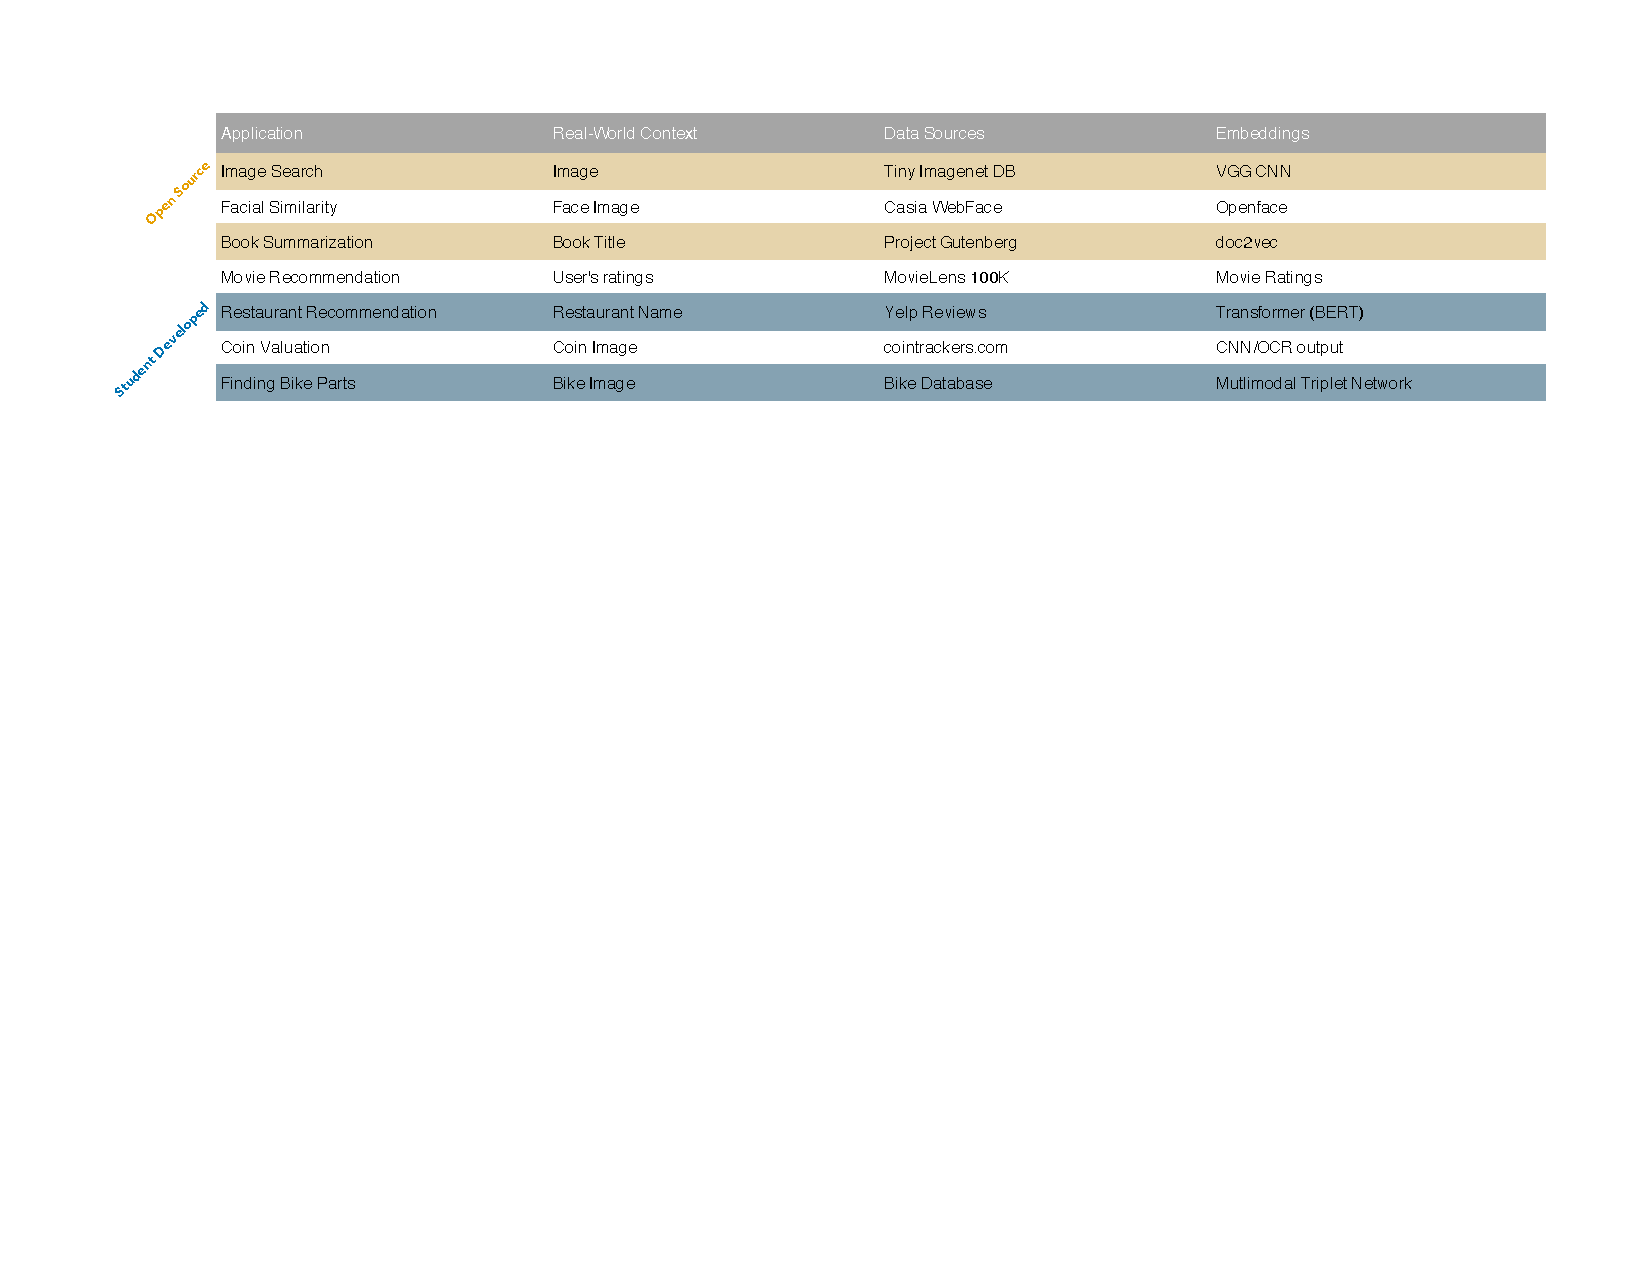
\includegraphics[width=\linewidth,]{figs/applications.pdf}
\begin{tabular}{|l|c|c|c|}
\hline
\textbf{APPLICATION} & \textbf{REAL-WORLD CONTEXT} &  \textbf{DATA SOURCES} & \textbf{EMBEDDINGS} \\ \hline
Image Search & Image & Tiny Imagenet DB & VGG CNN \\ \hline
Facial Similarity & Face Image & Casia WebFace & Openface \\ \hline
Book Summarization & Book Title & Project Gutenberg & doc2vec \\ \hline
Movie Recommendation & User's ratings & MovieLens 100K & Movie Ratings \\ \hline
Restaurant Recommendation & Restaurant Name & Yelp Reviews & Transformer (BERT) \\ \hline
Coin Valuation & Coin Image & cointrackers.com & CNN/OCR output \\ \hline
Finding Bike Parts & Bike Image & Bike Database & Mutlimodal Triplet Network \\ \hline
\bottomrule
\end{tabular}
    \vspace{0.05cm}
    \caption{A table of applications implemented in Quill. The datasets pertaining to the Data Sources for Existing applications are Tiny Imagenet \cite{le2015tiny}, CASIA WebFace \cite{yi2014learning}, Project Gutenberg \cite{lahiri:2014:SRW}, and MovieLens 100K \cite{harper2015movielens}.}
    \label{table:applications}
    % \vspace{-0.5cm}
\end{table*}



\section{Experiments}
\label{sec:evaluation}
We evaluate Quill in terms of usability~(is development with Quill easy?), performance~(are applications developed with Quill performing acceptably?), and modularity/adaptability~(can Quill adapt to advancements surrounding real-world data enrichment?).
To evaluate performance, we compare the latency of the original implementations of existing applications described in Table \ref{table:applications} with the Quill implementations.
We then discuss how to address retrieval accuracy while using Quill and the accuracy vs. latency trade-off.
Our evaluation of usability considers how succinct and expressive the DSL is, as well as how usable it is as reported by the student developers who developed applications using it.
The usability is also proven in the succinctness of scripts written in our DSL.
We demonstrate the adaptability of Quill by utilizing embedding functions learned from Ember \cite{suri2021ember}, a separate framework for keyless joins, and showing that Quill performs comparably to the keyless join from Ember, with added flexibility.\vspace{0.1cm}

\paragraph{Applications:}
\label{sec:evaluation:apps}
Quill's performance is evaluated against four existing applications, while the usability of Quill is evaluated using three novel applications developed by student developers. The applications are summarized in Table \ref{table:applications}.
Each application aims to complete a task that could be adapted to a multi-modal AR context. The image search application joins images from possibly two different modalities to return relevant images. The facilial similarity application is similar but restricted to facial images.
The Book summarization application joins a book title~(possibly obtained via the digitization of a book cover in the wild) and a topic with the full text of that book in order to provide of summary.
The movie recommendation application joins a set of user ratings of movies with a dataset of movies and previous ratings in order to recommend movies to the user.
The restaurant recommendation application joins a restaurant name~(possibly digitized from the real world) with Yelp reviews in order to find similar restaurants in the area.
The coin valuation application joins a coin image captured from the real world with a database of coin values to predict the value of the coin.
The finding bike parts application joins a bike image with a bike database to let a user know where to find replacement parts.\looseness=-1\vspace{0.1cm}

\paragraph{Experimental Datasets:}
\label{sec:evaluation:datasets}
To compare the Quill implementations of existing projects to the original implementations, we use the data sets mentioned in the documentation of the projects obtained from GitHub when possible.
The datasets used for measuring latency in each existing project are listed in the Data Sources column of Table~\ref{table:applications}.
To measure accuracy using the book summarization application, we use the WikiPassageQA \cite{cohen2018wikipassageqa} question answering dataset.

\subsection{Performance Evaluation}
\label{sec:evaluation:perf}
Quill should produce apps that return data that enriches the real world promptly to enable the development of apps that can interactively enrich the real world.
Consequently, Quill's performance evaluation is concerned with the latency of ARK-joins and how latency is affected at scale.
Additionally, applications built with Quill should provide relevant results to the user.
As a baseline for performance, we use the open-source projects described above.
We describe the Quill implementations of these projects before presenting their performance evaluation results.\looseness=-1\vspace{0.1cm}

\paragraph{Implementations:}
\label{sec:evaluation:implementations}
The process described in Section~\ref{sec:developing} was used to implement each of the existing projects in Quill.
For all the implementations, we use the IVF indexing method described in Section~\ref{sec:implementation:server} to store embeddings.
The number of centroids used in the indexing method is set to the square root of the number of stored data instances.
The locality of the embedding stores relative to the machine running the Quill app was made to match the locality of the embeddings used in the original implementations.\vspace{0.1cm}

\paragraph{Latency:}
\label{sec:evaluation:latency}
For each application, we measure latency as a function of the size of the data sets we join against.
Figure \ref{fig:latencies} shows results.
Our goal is to demonstrate that applications built with Quill perform ARK-joins more efficiently and in a more scalable manner than those built without Quill.
For each experiment, we select a random sample of the desired size from the corresponding data set for use by the baseline and the Quill implementation.\vspace{0.1cm}

Figure \ref{fig:latencies} shows the latency of the original~(or baseline) implementations of the applications compared to Quill implementations.
For reference, the plot for the facial similarity application contains a line for the Quill implementation using a ``full probe'', meaning that a single centroid was used across the board, which equates to an exhaustive search on the embedded vectors.
Quill beats all the baselines at scales greater than 10,000 data instances and grows at rates slower than those observed in the baseline implementations.
The improvement in performance at scale comes from our use of indexing for ANN search, which processes only a portion of the data set instead of all data instances.
However, we can see from the full probe results of the facial similarity example that even when a true nearest neighbor is retrieved instead of an approximate one, Quill outperforms the baseline.
The baseline outperforms Quill on some very small data sizes, which is due to overhead surrounding embedding stores that would not be necessary for data sizes this small.
Quill largely outperforms the book summarization baseline due to non-optimal programming practices leading to unnecessary computation such as training the embedding function every time a query is made.
Using our DSL, developers can more reliably produce performant applications by avoiding anti-patterns such as retraining.
Additionally, users benefit from the approximation modules built into Quill that can otherwise be difficult to utilize.
\vspace{0.1cm}

\begin{figure*}[ht]
  \begin{tabular}{cc}
    % \toprule
    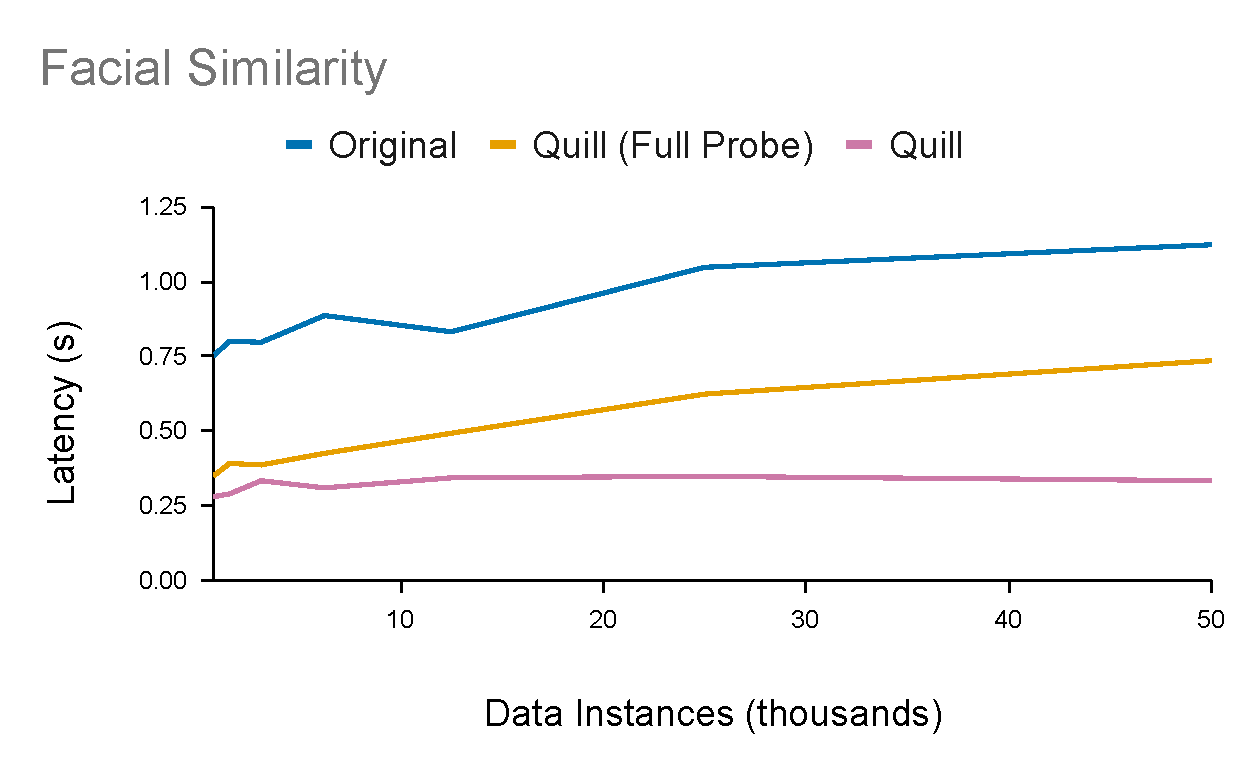
\includegraphics[width=0.5\linewidth]{figs/openface_latency_large.pdf} & 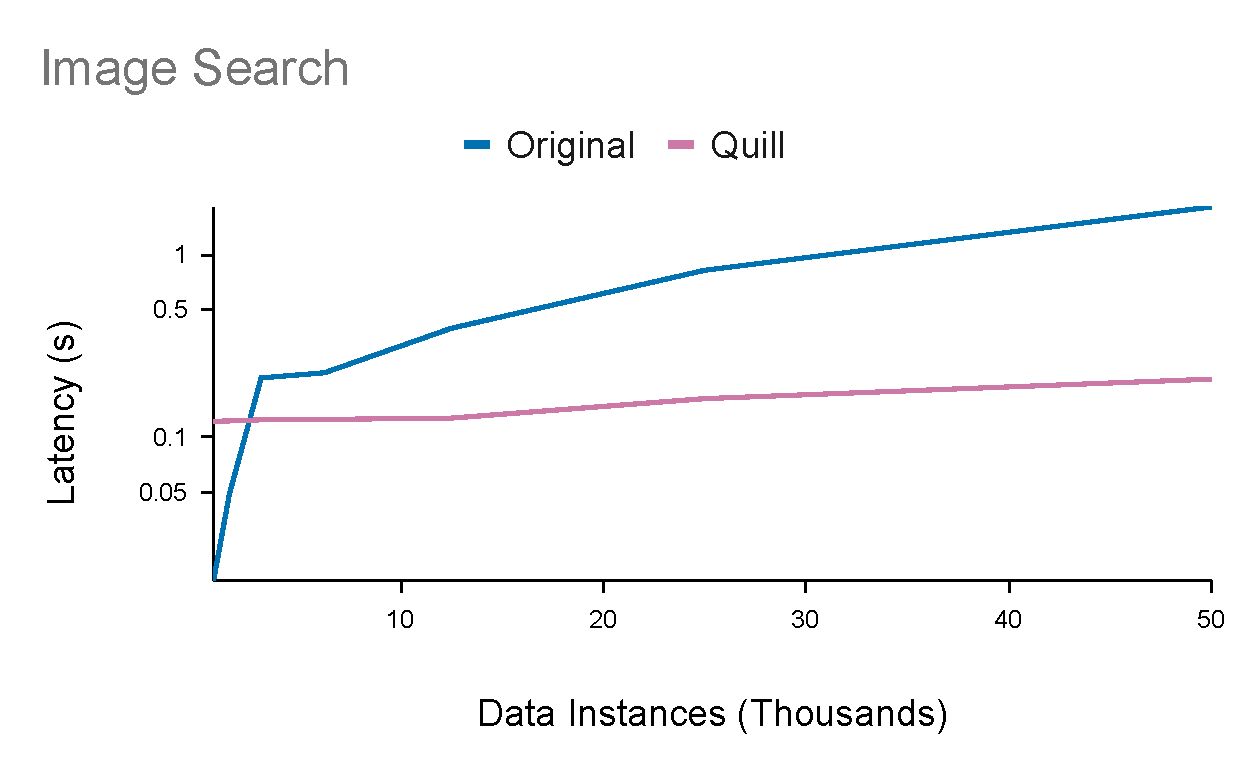
\includegraphics[width=0.5\linewidth]{figs/imagesearch_latency_large.pdf} \\
    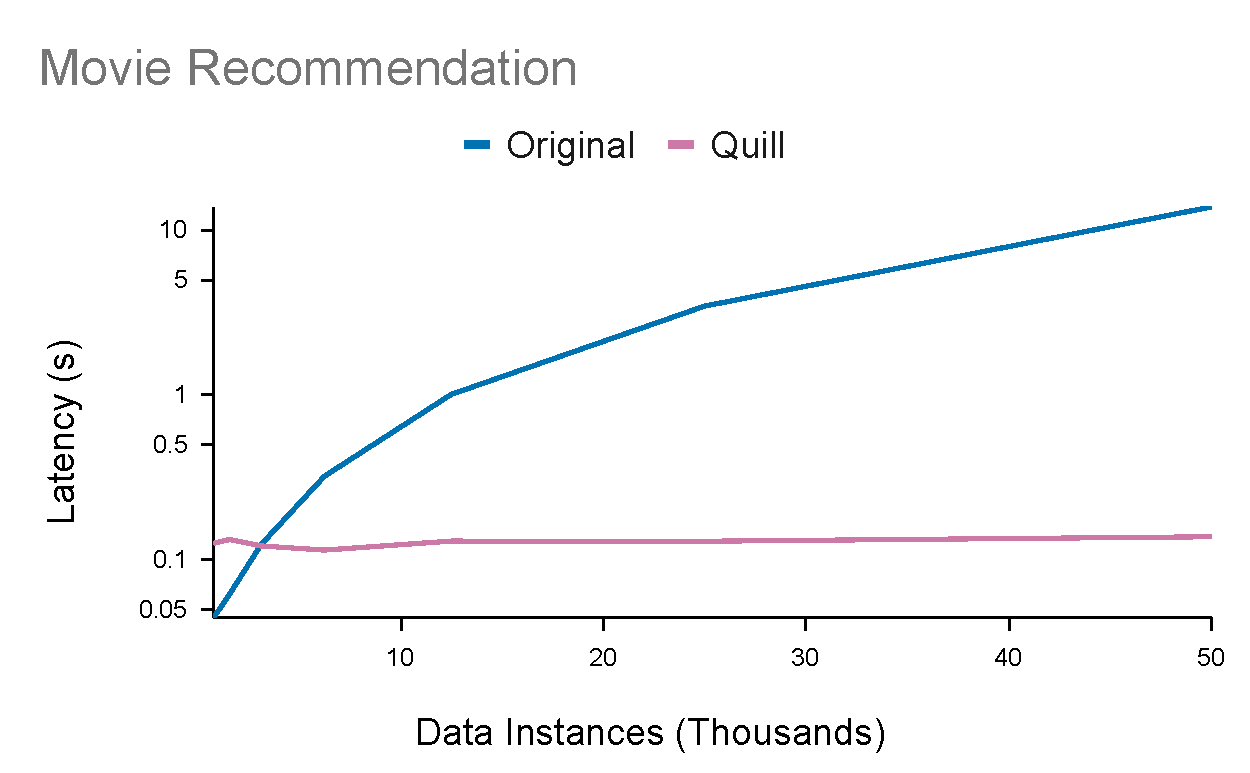
\includegraphics[width=0.5\linewidth]{figs/movie_latency_large.pdf}  & 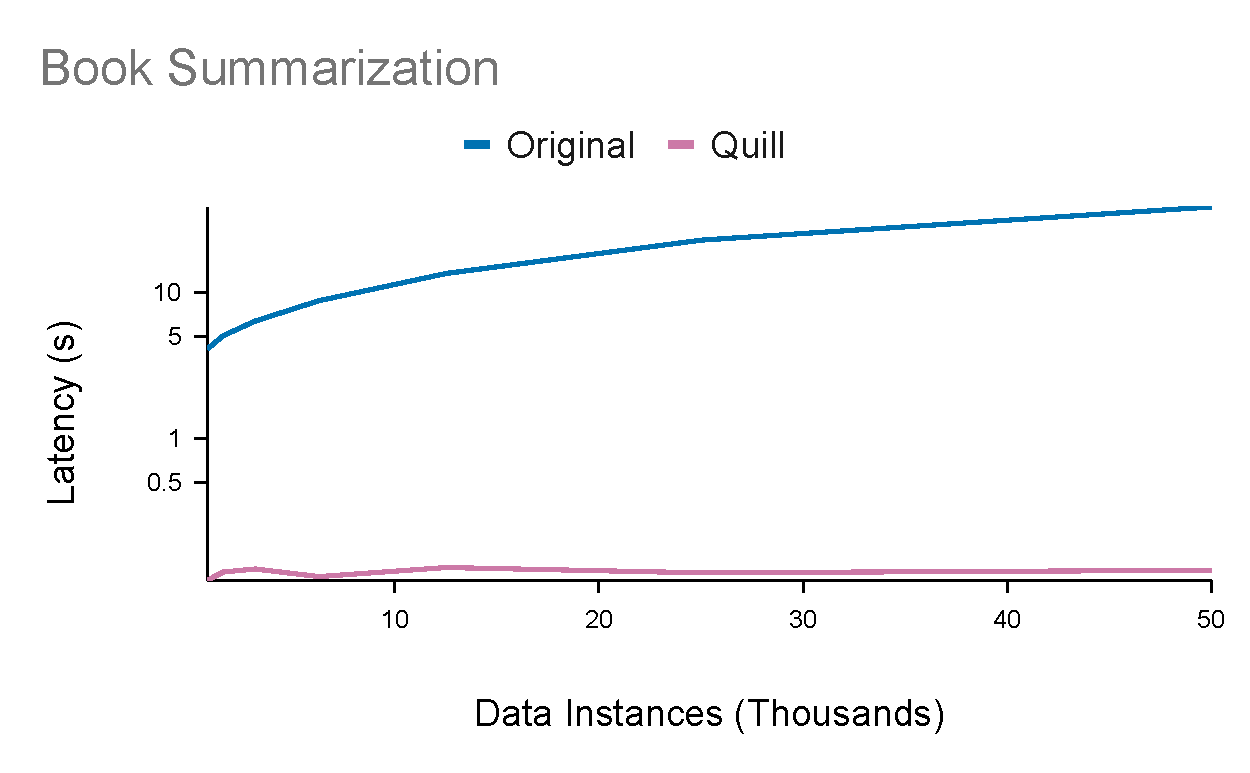
\includegraphics[width=0.5\linewidth]{figs/booksummarization_latency_large.pdf} \\ 
    % \bottomrule
  \end{tabular}
  \caption{For each of the four existing projects we implement, we record the latency as a function of data size.}
  \label{fig:latencies}
\end{figure*}

\paragraph{Accuracy:}
\label{sec:evaluation:accuracy}
When developing an application that joins on the real world, it is paramount that relevant results are presented.
Real-world decisions made with irrelevant information are fated to have negative or unexpected real-world consequences.
The requirement for accuracy goes hand in hand with the requirement for latency.
Joined results returned after the time they are needed are useless.
Quill enables developers to tune the trade-off between latency and accuracy in their applications.
Quill does this by exposing indexing parameters through the configuration file for the Quill application~(project.yaml) or the embedding store expression of a QWL specification.
For example, the IVF indexing method is parameterized by the number of centroids used for clustering.
Along with the indexing configuration, the quality of retrieval depends on the embedding function and distance metric used.
Quill enables developers to integrate customized versions or use off-the-shelf methods seamlessly in its framework.

We demonstrate the change in accuracy with respect to the number of centroids for the IVF indexing method in Figure \ref{fig:accuracy}.
We use mean average precision, mean reciprocal rank, and recall at 5, 10, and 20 when evaluating the accuracy.
The retrieval quality metric that is important is application dependent, and these metrics cover a wide spectrum that allows us to demonstrate that ARK-Join accuracy is tunable within a Quill app.
We measured the retrieval-based metrics by adding a \texttt{Context} expression to the book summarization application that takes in the number of desired centroids and utilizing that number in the embedding store expression to configure the number of centroids.
As expected, as the number of centroids increases, the quality of retrieval goes down.

\begin{figure}[ht]
  \centering
  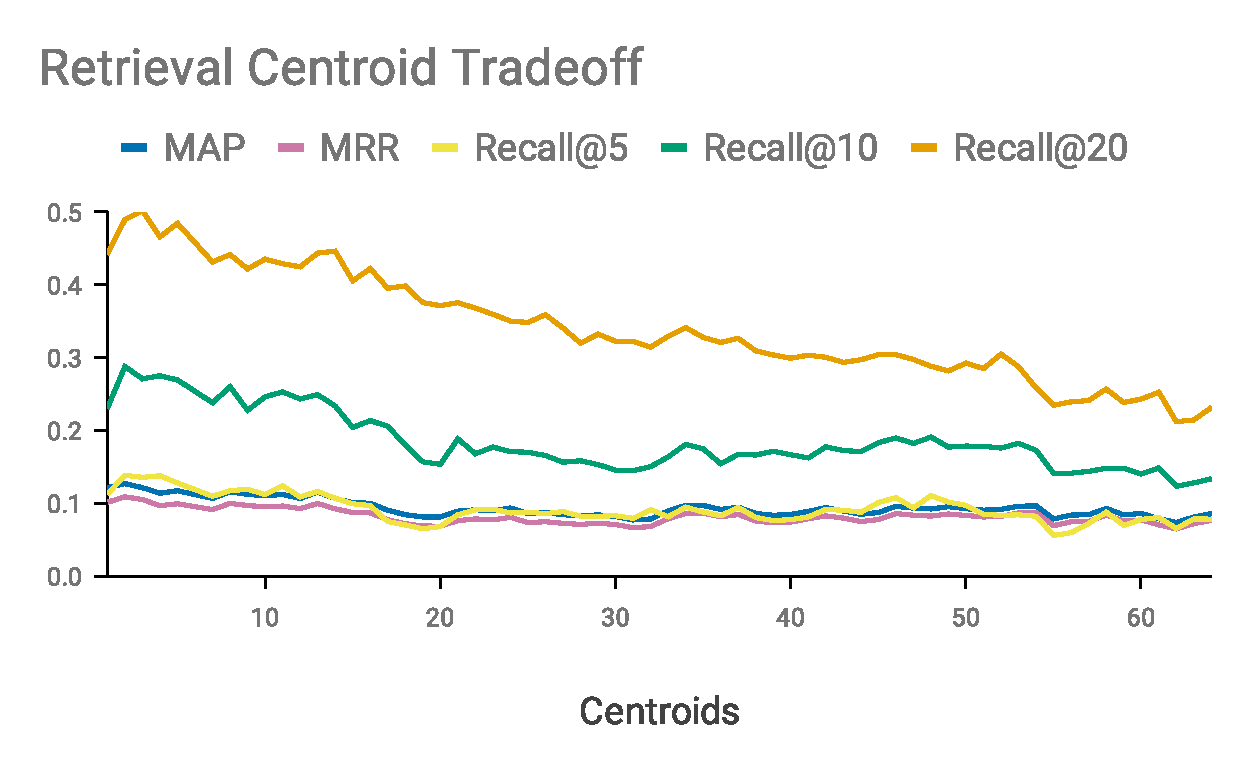
\includegraphics[width=0.6\linewidth]{figs/accuracy_large.pdf}
  \caption{Using the book summarization application on the WikiPassageQA dataset we measure mean average precision~(MAP), mean reciprocal rank~(MRR), and recall at 5, 10, and 20 as a function of the number of centroids used in the IVF indexing of the embedded data. \looseness=-1}
  \label{fig:accuracy}
\end{figure}


\subsection{Modularity}
\label{sec:evaluation:modularity}
\begin{figure}
  \centering
  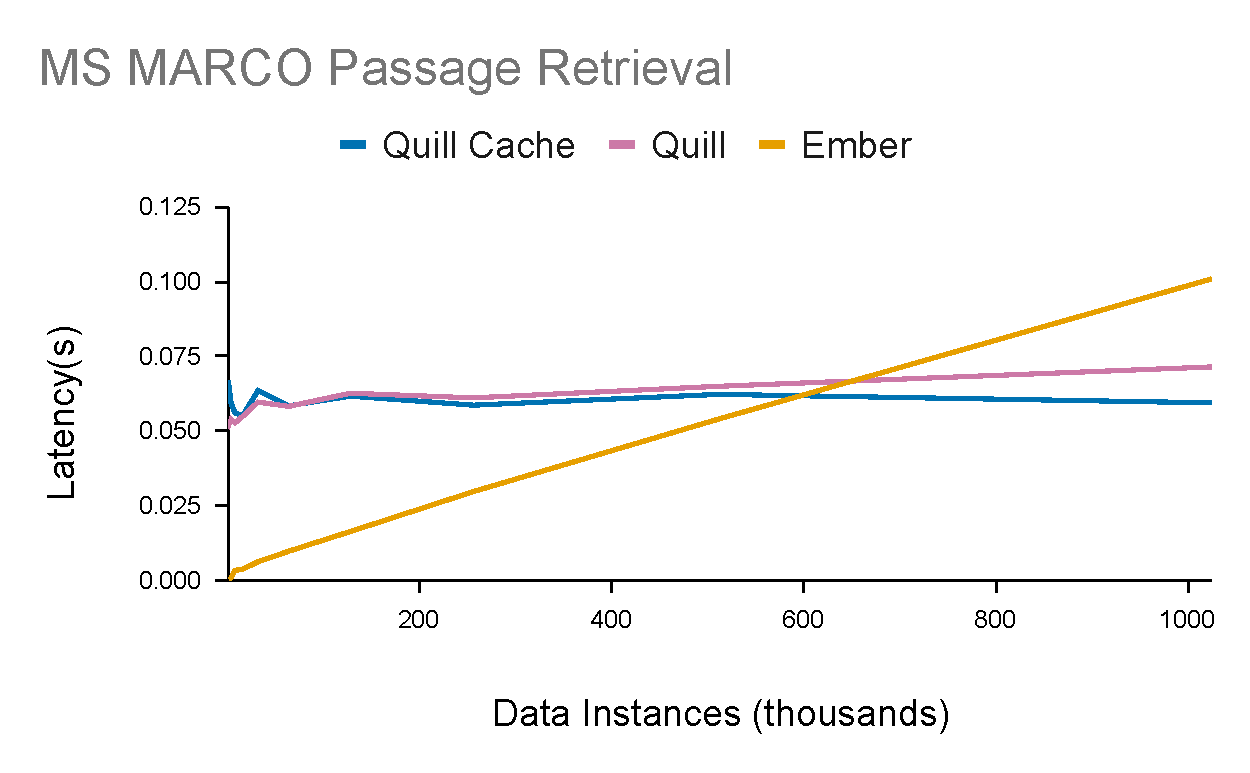
\includegraphics[width=0.6\linewidth]{figs/msmarco_large.pdf}
  \caption{Using passages from the MS MARCO dataset \cite{msmarco}, we compare the performance of the keyless join from Ember \cite{suri2021ember} with the ARK-join from two Quill applications: one with a low-latency cache, and one without a cache. \looseness=-1}
  \label{fig:msmarco}
\end{figure}

The foundation of Quill is the ARK-join-centered grammar we defined in Section~\ref{sec:grammar}.
This grammar should be modular enough to ensure that Quill can adapt to new technologies surrounding real-world joins, such as new embedding techniques.
Thus to demonstrate the modularity of Quill, we evaluate the performance of a passage retrieval application developed in Quill that utilizes an embedding function from a state-of-the-art framework for keyless joins, Ember \cite{suri2021ember}.
By showing that Quill can utilize this embedding method while outperforming a state-of-the-art keyless join, we establish that Quill is modular.

Using an open-source implementation of Ember, we compare the latency of the Ember keyless join with that of the ARK-joins from two Quill applications: one with a low latency cache and another without a cache.
We measure latency on the MS MARCO passage retrieval dataset which contains a set of passages obtained from web pages pertaining to a sample of Bing queries \cite{msmarco}.
The Ember keyless join and the Quill app without a cache both assume a 40 ms cloud-store communication latency.
The caching Quill app simulates an application deployed in a local caching architecture similar to Figure \ref{fig:edge-cache}, and doesn't incur the communication latency when the cache is utilized.
We configure the caching Quill app to use a similarity threshold that produces a cache hit ratio of 0.2.
Because we are using identical embedding functions~(obtained from Ember), we do not include the time to embed in our profiling of the join functions, which explains the difference in latency measurements observed in Section~\ref{sec:evaluation:latency} and the measurements observed here. Figure \ref{fig:msmarco} shows results.\vspace{0.1cm}

\paragraph{Discussion:}
We note that Ember's keyless join uses an exhaustive maximum inner product search, while we use an approximate search.
This results in the linear growth in latency for Ember that is not seen by Quill.
The same accuracy and latency would be seen from Quill when the indexing of the embedding store is configured to be exhaustive.
This emphasizes the flexibility of Quill to accommodate different accuracy and latency requirements.
The low latency achieved by the caching Quill app emphasizes Quill's ability to adapt to different architectures for further performance improvements.

By abstracting the embedding function as a user-provided function, Quill can utilize future advances surrounding real-world data enrichment.
This is demonstrated in our evaluation here which uses an embedding function learned from a state-of-the-art framework for keyless joins.
Quill seamlessly utilizes this embedding function while providing flexibility with respect to performance and application architecture.

% \begin{figure}[ht]
%   \centering
%   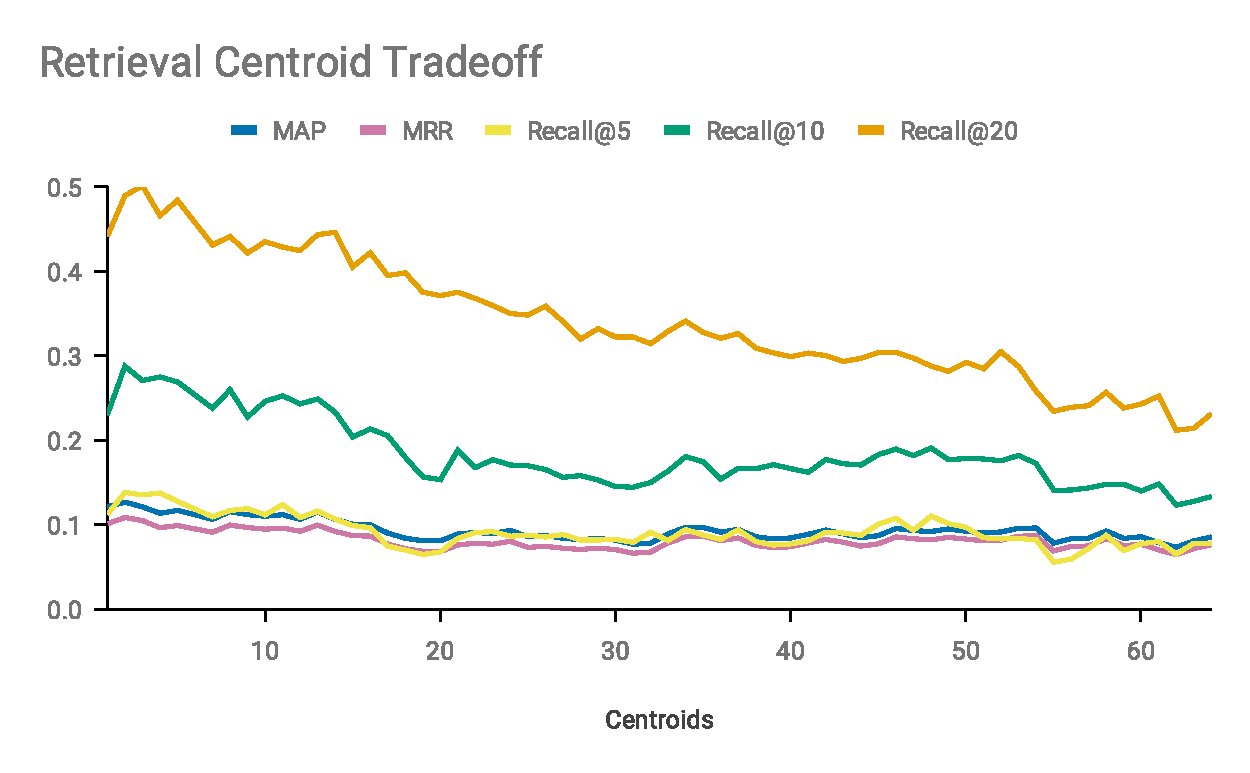
\includegraphics[width=0.6\linewidth]{figs/accuracy.pdf}
%   \caption{Using the book summarization application on the WikiPassageQA dataset we measure mean average precision~(MAP), mean reciprocal rank~(MRR), and recall at 5, 10, and 20 as a function of the number of centroids used in the IVF indexing of the embedded data. \looseness=-1}
%   \label{fig:accuracy}
% \end{figure}

\subsection{Usability}
\label{sec:evaluation:usability}
Quill provides a development framework that alleviates the effort currently required to produce an AR application that enriches real-world data.
In order to measure the usability of Quill's DSL, we perform user studies by asking student developers to write an application of their choosing using a Pythonic dialect of QWL. We recruited three college students between the ages of 19 and 28, ranging in Python proficiency from little to significant experience. Two out of these three student developers had beginner-level experience with various concepts of applied machine learning. We measure the overall usability of Quill's DSL via results from the system usability scale~(SUS) \cite{brooke1996sus}.
The SUS consists of 10 Likert scale questions and is an industry standard for measuring system usability.
We also report findings on the succinctness of the Quill implementation of existing projects.\looseness=-1\vspace{0.1cm}

\paragraph{Test Setup:}
\label{sec:evaluation:usable}
Each student was provided a one-on-one tutorial on QWL.
The content presented to the students was identical, minus any questions asked.
At the end of the tutorial, students were asked to describe their application using a DAG of elements from our grammar described in Section~\ref{sec:grammar}.
The number of iterations required during this process is elaborated in the discussion.
When a student was happy with their application description, and it was confirmed valid by the proctor, they moved on to writing the QWL code.
We provided documentation and sample QWL scripts for reference.
We asked students to bring a laptop with their text editor of choice to write the QWL code.
The number of iterations required to produce a valid QWL script was recorded.
Concluding the study, we asked students to complete the SUS survey.\vspace{0.1cm}

\paragraph{User Study Results:}
Throughout our discussion of the user studies, we refer to the students as A, B, and C, who developed the coin valuation app, the restaurant recommendation app, and the bike parts app respectively.
All of the students completed their valid DAG of grammar elements in a single iteration without help from the proctor.
Like the DAGs, QWL scripts for all students' applications were completed in a single iteration without help.
While questions were asked during the tutorials, there were no questions needed to create the DAGs or QWL scripts. Each student in this study took the system usability scale based on their experience with QWL.
Results are shown in table \ref{table:sus}.
QWL scored an average of 68.33.
Studies show that scores of 68 and above are considered good \cite{brooke1996sus, bangor2008empirical}, implying QWL scores well in terms of usability.
In addition to the SUS results, we found that the Quill implementations of existing projects used in our performance evaluation were more succinct, using 30\% less lines of code on average.

\paragraph{Maintaining Performance alongside Usability:}
The Quill framework must produce performant applications while remaining usable. In this section, we demonstrated that Quill is usable, and in Section~\ref{sec:evaluation:perf}, we showed that Quill produces performant applications. The balance between usability and performance is made possible by allowing the underlying framework to handle the complexities of applications that join real-world data. Quill prevents developers from falling into the traps of anti-patterns such as retraining; developers provide the embedding models, and Quill decides how to use them. Our implementation of the ARK-join handles many optimizations that lead to clumsy code when done by hand, such as indexing for approximate nearest neighbor operations. Moreover, Quill uses efficient approximation modules that can be difficult for the lay user to utilize.

\begin{table}[ht]
\begin{tabular}{|p{0.75\columnwidth}|c|}
\hline
\textbf{QUESTION} & \textbf{AVERAGE} \\ \hline
I would like to use this frequently & Agree \\ \hline
The system was easy to use & Neutral \\ \hline
The various functions in this system were well integrated & Agree \\ \hline
Most people would learn to use this system very quickly & Agree \\ \hline
I felt very confident using this system & Neutral \\ \hline
I found the system unnecessarily complex & Disagree \\ \hline
I would need the support of a technical person to use this & Disagree \\ \hline
There was too much inconsistency with this system & Disagree \\ \hline
The system is cumbersome to use & Disagree \\ \hline
I need to learn a lot of things before using this system & Disagree \\ \hline
\bottomrule
\end{tabular}
\vspace{0.05cm}
\caption{Results of a Systems Usability Survey on student developers. Results suggest that Quill scores well in terms of usability}
\label{table:sus}
\end{table}

\subsection{Discussion}
Our evaluation of Quill demonstrates its ability to simply define complex ARK-join functionality to produce robust, scalable applications.
As demonstrated by the latency results of the image search application in Figure \ref{fig:latencies}, it is possible that, for applications with small amounts of data, a non-Quill implementation can provide better results.
Here it should be noted that Quill is more generalized than highly application-specific solutions that do not extend to other use cases. Optimizing to reduce latency for small data sizes is considered future work. After taking the SUS, we asked the developers to provide free form feedback about their experience using QWL.
One developer expressed, ``My only concern would be making the embedding fit the scope of the expected data so the ARK-Join can return proper results however that is not the goal of the project and relies on development from the user.’’
This reiterates what we stated previously.
Quill provides a flexible way to utilize off-the-shelf as well as custom embedding functions and indexing techniques in a single development framework, as the quality of retrieval is largely dependent on the embedding and indexing methods used by the developer.
Another developer remarked, ``I can not think of why I would use a non-closest neighbor join condition. But I can think of reasons to multiply the differences by a vector of attribute weights~(i.e., non-euclidean distance)’’.
This student refers to the way ARK-Joins are defined in QWL: the developer provides a predicate for the join, which is often a nearest neighbor-based predicate.
While the student may be suggesting that we assume the condition will always be the nearest neighbor operation, we did not make this assumption to allow for classical join predicates.



\section{Related Work}

\subsection{Interactive Data Systems for AR} The main idea of interactive data systems in AR revolves around bringing data to the real world in a way that allows users to enhance their view of reality. Earlier works in this domain, such as AR web-browsers, attempt to bring together data from multiple sources to create such an experience. Argon \cite{macintyre2011argon} is one such architecture that brings together multiple separately authored AR applications~(built using their KHARMA \cite{hill2010kharma} framework) into one browser view.
While this platform does bring multiple data sources into the real world, it exclusively supports sensor and marker-based AR.
Quill provides marker-less AR in which experiences are determined based on semantic relationships.
The performance requirement of interactive data systems for AR poses a challenge to the development of such systems. Schneider et at. \cite{schneider2017augmented} utilize edge computing technologies to allow AR applications to offload some of the computationally heavy tasks associated with AR. Their work focuses on offloading tasks common across AR applications, while Quill focuses on improving performance in the context of real-world data understanding and enrichment.

\subsection{Keyless Joins} Recent works on keyless joins have proven them useful where similarity-based joins are needed and defining similarity functions explicitly is unreasonable.
Ember \cite{suri2021ember} uses transformer-based machine learning techniques to learn similarity functions for joins used in context enrichment in machine learning pipelines.
Termite \cite{fernandez2019termite} uses Siamese networks to learn similarity functions to aid in data integration tasks on heterogeneous text-based structured and unstructured data.
These works learn keyless joins in frameworks that operate on modalities of data present in their respective tasks~(ML context enrichment and text-based data integration).
In contrast, Quill abstracts the similarity function of our keyless join~(ARK-join) as a parameter to enable Quill apps that operate on varying modalities of data.
Additionally, Quill's ARK-join can adapt to state-of-the-art learned similarity functions.

\subsection{Semantic representation of relational data stores} The desire to link datasets based on \emph{semantic} information has given rise to work that utilizes learned embeddings to represent structured data in a semantic vector space.
The work titled Cognitive Databases \cite{bordawekar2017cognitive} represents relational data as unstructured text in order to utilize word embeddings to represent the relational data as a vector.
Similarly, Cappuzzo et al.~\cite{cappuzzo2020creating} create embeddings of relational data for data integration by representing the data using a graph which allows them to use graph embedding techniques.
We benefit from these works by utilizing methods they describe to embed relational data sets.
Fernandez et al.~\cite{fernandez2018seeping} utilize word embeddings in order to find links within datasets semantically. In their recent work \cite{fernandez2019termite} called Termite, they used embedding techniques to perform data integration for various relational data stores.
The additional constraint Quill imposes on its operation is the capability of handling multimodal real-world data as well as heterogeneous relational database schema within the interactive latency imposed by AR interfaces.

\section{Conclusion and Future Work}

Increasing advancement of technology in key related areas has made sure that widespread use of augmented reality~(AR) is an inevitability rather than a distant possibility. While the necessary computing resources and technology needed to make immersive AR applications have become more readily available, developing a performant AR application that enriches real-world data with digital information is still a challenging task. Quill makes it easier to develop immersive AR applications that make it easier for the user to gather insights from real-world data by using an expressive DSL backed by an intuitive grammar. Quill serves as a natural extension of ARQuery \cite{burley2019arquery} by enabling join queries specified using ARQuery to utilize remote data to enhance data in the real world. We demonstrate that Quill's development framework not only makes it easier to develop data-rich AR applications for developers with limited background knowledge in related technical areas, but it also produces more performant applications than other existing developer tools. Looking forward, we realize that although Quill accelerates the development workflow for AR applications, it only addresses a small portion of the problems surrounding the development of AR applications that enhance a user's view of real-world data.
For example, sharing a user's enhanced view of real-world data within an interactive, AR-enabled interface to her friends on social media in a scalable way is an important piece of future work. To what extent an AR-enabled application should alter a user's view of the real world also requires a closer look at the underlying problem, as if done wrong it can have serious adverse consequences.
Additionally, we hope to improve the performance of Quill apps by intelligently placing caching and indexing on the edge in a declarative manner similar to Shaowang et al. \cite{shaowang2021declarative}.
We hope to address these problems in our future works as more advances are made in democratizing the development of AR applications empowered by a vibrant larger-than-ever developer community.

\section*{Acknowledgement}
This material is based upon work supported by the National Science Foundation under Grant No. 1910356.

\begin{thebibliography}{10} 
\itemsep=1pt 
\begin{small}

\bibitem{azuma2001recent} Ronald Azuma, Yohan Baillot, Reinhold Behringer, Steven Feiner, Simon Julier, and Blair MacIntyre. 2001. Recent Advances in Augmented Reality. IEEE CG\&A
(2001).

\bibitem{burley2019arquery} Codi J Burley and Arnab Nandi. 2019. ARQuery: Hallucinating Analytics over Real-World Data using Augmented Reality. In CIDR.

\bibitem{nandi2013gestural} Arnab Nandi, Lilong Jiang, and Michael Mandel. 2013. Gestural Query Specification. VLDB (2013).


\bibitem{fernandez2018seeping} Raul Castro Fernandez, Essam Mansour, Abdulhakim A Qahtan, Ahmed Elmagarmid, Ihab Ilyas, Samuel Madden, Mourad Ouzzani, Michael Stonebraker, and Nan Tang. 2018. Seeping semantics: Linking datasets using word embeddings for data discovery. In 2018 IEEE 34th International Conference on Data Engineering (ICDE). IEEE, 989–1000.

% \bibitem{tang2020cooperative} Sihai Tang, Bruce Haidi Chen, Jacob Hochstetler, Jason Hirsch, and Song Fu. 2020. Cooperative Mixed Reality Leveraging Edge Computing and Communication. In 2020 IEEE/ACM Symposium on Edge Computing (SEC). IEEE, 425–429.

% \bibitem{drolia2017cachier} Utsav Drolia, Katherine Guo, Jiaqi Tan, Rajeev Gandhi, and Priya Narasimhan. 2017. Cachier: Edge-Caching for Recognition Applications. In 2017 IEEE 37th International Conference on Distributed Computing Systems (ICDCS). 276–286. https://doi.org/10.1109/ICDCS.2017.94

% \bibitem{li2017mobiqor} Yongbo Li, Yurong Chen, Tian Lan, and Guru Venkataramani. 2017. MobiQoR: Pushing the Envelope of Mobile Edge Computing Via Quality-of-Result Optimization. In 2017 IEEE 37th International Conference on Distributed Computing Systems (ICDCS). 1261–1270. https://doi.org/10.1109/ICDCS.2017.54

% \bibitem{ren2018mobile} Pei Ren, Xiuquan Qiao, Junliang Chen, and Schahram Dustdar. 2018. Mobile edge computing–a booster for the practical provisioning approach of web-based augmented reality. In 2018 IEEE/ACM Symposium on Edge Computing (SEC). IEEE, 349–350.


\bibitem{sarkhel2019deterministic} Ritesh Sarkhel and Arnab Nandi. 2019. Deterministic Routing between Layout Abstractions for Multi-Scale Classification of Visually Rich Documents. In IJCAI. 3360–3366.

\bibitem{sarkhel2019visual} Ritesh Sarkhel and Arnab Nandi. 2019. Visual Segmentation for Information Extraction from Heterogeneous Visually Rich Documents. In Proceedings of the 2019 International Conference on Management of Data. ACM, 247–262.

\bibitem{sarkhel2021improving} Ritesh Sarkhel and Arnab Nandi. 2021. Improving information extraction from visually rich documents using visual span representations. Proceedings of the VLDB Endowment 14, 5 (2021), 822–834.

\bibitem{suri2021ember} Sahaana Suri, Ihab F Ilyas, Christopher Ré, and Theodoros Rekatsinas. 2021. Ember: No-Code Context Enrichment via Similarity-Based Keyless Joins. arXiv preprint arXiv:2106.01501 (2021).

\bibitem{fernandez2019termite} Raul Castro Fernandez and Samuel Madden. 2019. Termite: a system for tunneling through heterogeneous data. arXiv preprint arXiv:1903.05008 (2019).

\bibitem{li2021auto} Peng Li, Xiang Cheng, Xu Chu, Yeye He, and Surajit Chaudhuri. 2021. Auto-FuzzyJoin: Auto-Program Fuzzy Similarity Joins Without Labeled Examples. In Proceedings of the 2021 International Conference on Management of Data. 1064– 1076.

\bibitem{afrati2012fuzzy} Foto N Afrati, Anish Das Sarma, David Menestrina, Aditya Parameswaran, and Jeffrey D Ullman. 2012. Fuzzy joins using mapreduce. In 2012 IEEE 28th International Conference on Data Engineering. IEEE, 498–509.

\bibitem{li2011pass} Guoliang Li, Dong Deng, Jiannan Wang, and Jianhua Feng. 2011. Pass-join:
A partition-based method for similarity joins. arXiv preprint arXiv:1111.7171
(2011).

\bibitem{metwally2012v} Ahmed Metwally and Christos Faloutsos. 2012. V-smart-join: A scalable mapreduce framework for all-pair similarity joins of multisets and vectors. arXiv preprint arXiv:1204.6077 (2012).

\bibitem{chen2019customizable} Zhimin Chen, Yue Wang, Vivek Narasayya, and Surajit Chaudhuri. 2019. Customizable and scalable fuzzy join for big data. Proceedings of the VLDB Endowment 12, 12 (2019), 2106–2117.

\bibitem{manning2008and} Christopher D Manning and Prabhakar Raghavan. 2008. Introduction to Information Retrieval. Cambridge University Press.

\bibitem{jens} Jens Dittrich and Alekh Jindal. 2011. Towards a One Size Fits All Database Architecture. CIDR (2011).

\bibitem{cavanagh2005tracking} Patrick Cavanagh and George A Alvarez. 2005. Tracking multiple targets with multifocal attention. Trends in cognitive sciences 9, 7 (2005), 349–354.

\bibitem{jegou2010product} Herve Jegou, Matthijs Douze, and Cordelia Schmid. 2010. Product quantization for nearest neighbor search. IEEE transactions on pattern analysis and machine intelligence 33, 1 (2010), 117–128.

\bibitem{carvalho2018cross} Micael Carvalho, Rémi Cadène, David Picard, Laure Soulier, Nicolas Thome, and Matthieu Cord. 2018. Cross-modal retrieval in the cooking context: Learning semantic text-image embeddings. In The 41st International ACM SIGIR Conference on Research \& Development in Information Retrieval. ACM, 35–44.

\bibitem{le2015tiny} Ya Le and Xuan Yang. 2015. Tiny imagenet visual recognition challenge. CS
231N (2015).

\bibitem{yi2014learning} Dong Yi, Zhen Lei, Shengcai Liao, and Stan Z Li. 2014. Learning face representation from scratch. arXiv preprint arXiv:1411.7923 (2014).

\bibitem{lahiri:2014:SRW} Shibamouli Lahiri. 2014. Complexity of Word Collocation Networks: A Preliminary Structural Analysis. In Proceedings of the Student Research Workshop at the 14th Conference of the European Chapter of the Association for Computational Linguistics. Association for Computational Linguistics, Gothenburg, Sweden,
96–105. http://www.aclweb.org/anthology/E14- 3011

\bibitem{harper2015movielens} F Maxwell Harper and Joseph A Konstan. 2015. The movielens datasets: History and context. Acm transactions on interactive intelligent systems (tiis) 5, 4 (2015), 1–19.

\bibitem{cohen2018wikipassageqa} Daniel Cohen, Liu Yang, and W Bruce Croft. 2018. Wikipassageqa: A benchmark collection for research on non-factoid answer passage retrieval. In The 41st International ACM SIGIR Conference on Research \& Development in Information Retrieval. 1165–1168.

\bibitem{msmarco} 2021. MS MARCO. https://microsoft.github.io/msmarco/

\bibitem{brooke1996sus} John Brooke. 1996. SUS: a ``quick and dirty'' usability. Usability evaluation in industry (1996), 189.

\bibitem{bangor2008empirical} Aaron Bangor, Philip T Kortum, and James T Miller. 2008. An empirical evaluation
of the system usability scale. Intl. Journal of Human–Computer Interaction 24, 6 (2008), 574–594.

\bibitem{macintyre2011argon} Blair MacIntyre, Alex Hill, Hafez Rouzati, Maribeth Gandy, and Brian Davidson. 2011. The Argon AR Web Browser and standards-based AR application environment. In 2011 10th IEEE International Symposium on Mixed and Augmented Reality. IEEE, 65–74.

\bibitem{schneider2017augmented} Michael Schneider, Jason Rambach, and Didier Stricker. 2017. Augmented reality based on edge computing using the example of remote live support. In 2017 IEEE International Conference on Industrial Technology (ICIT). IEEE, 1277–1282.

\bibitem{bordawekar2017cognitive} Rajesh Bordawekar, Bortik Bandyopadhyay, and Oded Shmueli. 2017. Cognitive database: A step towards endowing relational databases with artificial intelligence capabilities. arXiv preprint arXiv:1712.07199 (2017).

\bibitem{cappuzzo2020creating} Riccardo Cappuzzo, Paolo Papotti, and Saravanan Thirumuruganathan. 2020. Creating embeddings of heterogeneous relational datasets for data integration tasks. In Proceedings of the 2020 ACM SIGMOD International Conference on Management of Data. 1335–1349.

\bibitem{hill2010kharma} Alex Hill, Blair MacIntyre, Maribeth Gandy, Brian Davidson, and Hafez Rouzati. 2010. Kharma: An open kml/html architecture for mobile augmented reality applications. In 2010 IEEE International Symposium on Mixed and Augmented Reality. IEEE, 233–234.

\bibitem{shaowang2021declarative} Ted Shaowang, Nilesh Jain, Dennis D Matthews, and Sanjay Krishnan. 2021. Declarative data serving: the future of machine learning inference on the edge. Proceedings of the VLDB Endowment 14, 11 (2021), 2555–2562.

\end{small} 
\end{thebibliography}

\end{document}
